\chapter{Automated Distribution of Quantum Algorithms}
\label{chap:Project}

\section{Implementing non-local CNOT gates}
\label{NonLocalGates}

In \S\ref{IntroDistributing}, we explained the proposal by~\citet{NonLocalCNOT} of how to implement a non-local gate. In their work, a single ebit could be used to implement multiple CNOTs only if they shared a common control wire, and no operation was applied on it between the CNOTs. We will now extend their results.

Our first extension comes from the fact that some of the 1-qubit gates from the Clifford+T set commute with the CNOT gate. This means that, if there are operations in between CNOTs, we may transform the circuit to an equivalent version where the CNOT gates are brought together. All of the relevant circuit transformations are shown in Figure~\ref{fig:pullRules}. As also shown in Figure~\ref{fig:pullRules}, some gates do not commute with CNOT, but we can still interchange them if we add an extra 1-qubit gate. %These can be checked by calculating the corresponding matrices of both sides and verifying they match.

\begin{figure}
\hspace*{-6mm}
\begin{tikzpicture}
  \node[font=\itshape] (textA) {\(\forall g\in\{Z,S,T\}\) at control wire};
  \node [below=-5mm of textA] (A) {
    \begin{tikzpicture}
      \node[inner sep=0pt] (c1) at (0,0) {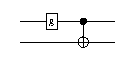
\includegraphics[scale=2]{Figures/circuits/C_gCNOT}};       
      \node[right=-13.9mm of c1.east, inner sep=0pt] (c2) {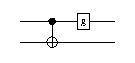
\includegraphics[scale=2]{Figures/circuits/C_CNOTg}};
      \node[right=-12mm of c1.east, rectangle, fill=white, minimum size=10mm] (eq) {\(=\)};  
      \node[right=7mm of c1.west, rectangle,fill=white,minimum width=5mm, minimum height=10mm] {};
      \node[left=7mm of c2.east, rectangle,fill=white,minimum width=5mm, minimum height=10mm] {};
    \end{tikzpicture}
  };
  \node[right=20mm of textA, font=\itshape] (textB) {\(\forall g\!\text{'}\in\{X,Y\}\) at control wire};
  \node [below=-5mm of textB] (B) {
    \begin{tikzpicture}
      \node[inner sep=0pt] (c1) at (0,0) {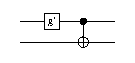
\includegraphics[scale=2]{Figures/circuits/C_g2CNOT}};       
      \node[right=-13.9mm of c1.east, inner sep=0pt] (c2) {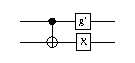
\includegraphics[scale=2]{Figures/circuits/C_CNOTg2}};
      \node[right=-12mm of c1.east, rectangle, fill=white, minimum size=10mm] (eq) {\(=\)};  
      \node[right=7mm of c1.west, rectangle,fill=white,minimum width=5mm, minimum height=10mm] {};
      \node[left=7mm of c2.east, rectangle,fill=white,minimum width=5mm, minimum height=10mm] {};
    \end{tikzpicture}
  };
  \node[below=20mm of textA, font=\itshape] (textC) {\(\forall g\in\{X\}\) at target wire};
  \node [below=-5mm of textC] (C) {
    \begin{tikzpicture}
      \node[inner sep=0pt] (c1) at (0,0) {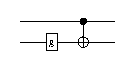
\includegraphics[scale=2]{Figures/circuits/T_gCNOT}};       
      \node[right=-13.9mm of c1.east, inner sep=0pt] (c2) {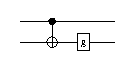
\includegraphics[scale=2]{Figures/circuits/T_CNOTg}};
      \node[right=-12mm of c1.east, rectangle, fill=white, minimum size=10mm] (eq) {\(=\)};  
      \node[right=7mm of c1.west, rectangle,fill=white,minimum width=5mm, minimum height=10mm] {};
      \node[left=7mm of c2.east, rectangle,fill=white,minimum width=5mm, minimum height=10mm] {};
    \end{tikzpicture}
  };
  \node[below=20mm of textB, font=\itshape] (textD) {\(\forall g\!\text{'}\in\{Y,Z\}\) at target wire};
  \node [below=-5mm of textD] (D) {
    \begin{tikzpicture}
      \node[inner sep=0pt] (c1) at (0,0) {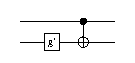
\includegraphics[scale=2]{Figures/circuits/T_g2CNOT}};       
      \node[right=-13.9mm of c1.east, inner sep=0pt] (c2) {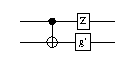
\includegraphics[scale=2]{Figures/circuits/T_CNOTg2}};
      \node[right=-12mm of c1.east, rectangle, fill=white, minimum size=10mm] (eq) {\(=\)};  
      \node[right=7mm of c1.west, rectangle,fill=white,minimum width=5mm, minimum height=10mm] {};
      \node[left=7mm of c2.east, rectangle,fill=white,minimum width=5mm, minimum height=10mm] {};
    \end{tikzpicture}
  };
\end{tikzpicture}
\caption{Different cases when a 1-qubit gate from Clifford+$T$ can be pushed through a CNOT gate.}
\label{fig:pullRules}
\end{figure}

The second improvement comes by realising that the method used to implement multiple CNOT gates controlled by the same wire can also be applied if multiple CNOTs have a common target qubit instead. We will refer to the former method as the \textit{remote-control} method, and to the latter as the \textit{remote-target} method. The derivation of the remote-target method is shown in Figure~\ref{fig:CNOTtargetProof}, which uses some of the properties listed in Figure~\ref{fig:props}.

\begin{figure}
\vspace*{11mm}
\hspace*{73mm}
\begin{tikzpicture}[transform canvas={scale=0.73}]
  \node (A) {
    \begin{tikzpicture}
      \node[inner sep=0pt] (c1) {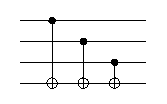
\includegraphics[scale=2]{Figures/circuits/proof1}};  
      \coordinate[below left=7mm and -6mm of c1.west] (l1);
      \coordinate[right=45mm of l1] (r1);
      \pic (cut1) {cut=l1/r1};     
      \node[right=0mm of c1] (eq1) {\Large \(=\)}; 
      \node[right=0mm of eq1, inner sep=0pt] (c2) {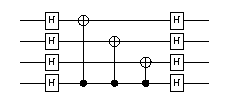
\includegraphics[scale=2]{Figures/circuits/proof2}};  
      \coordinate[below left=7mm and -6mm of c2.west] (l2);
      \coordinate[right=66mm of l2] (r2);
      \pic (cut2) {cut=l2/r2};  
      \node[right=0mm of c2] (eq2) {\Large \(=\)};  
    \end{tikzpicture}
  };
  \node[below=5mm of A] (B) {
    \begin{tikzpicture}
      \node (eq2) {\Large \(=\)};    
      \node[right=-4mm of eq2, inner sep=0pt] (circuit) {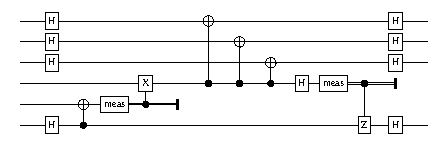
\includegraphics[scale=2]{Figures/circuits/proof3}};  
      \pic (e3) {ebit=e3/26.79mm/13mm};  
      \coordinate[below left=7mm and -6mm of circuit.west] (l3);
      \coordinate[right=140mm of l3] (r3);
      \pic (cut3) {cut=l3/r3};  
      \node[right=0mm of circuit] (eq3) {\Large \(=\)}; 
    \end{tikzpicture}
  };
  \node[below=5mm of B] (C) {
    \begin{tikzpicture}
      \node (eq3) {\Large \(=\)}; 
      \node[right=0mm of eq3, inner sep=0pt] (circuit) {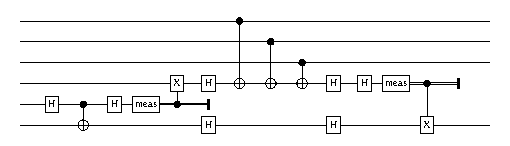
\includegraphics[scale=2]{Figures/circuits/proof4}};   
      \pic (e4) {ebit=e4/26.79mm/13mm};  
      \coordinate[below left=7mm and -6mm of circuit.west] (l4);
      \coordinate[right=161mm of l4] (r4);
      \pic (cut4) {cut=l4/r4};  
      \node[right=0mm of circuit] (eq4) {\Large \(=\)}; 
    \end{tikzpicture}
  };
  \node[below=5mm of C] (D) {
    \begin{tikzpicture}
      \node (eq4) {\Large \(=\)};    
      \node[right=-4mm of eq4, inner sep=0pt] (circuit) {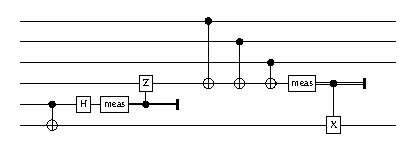
\includegraphics[scale=2]{Figures/circuits/proof5}};     
      \pic (e5) {ebit=e5/26.79mm/13mm};  
      \coordinate[below left=7mm and -6mm of circuit.west] (l5);
      \coordinate[right=129mm of l5] (r5);
      \pic (cut5) {cut=l5/r5};  
      \node[right=-4mm of circuit] (eq5) {\Large \(=\)};    
      \node[right=-4mm of eq5, inner sep=0pt] (c6) {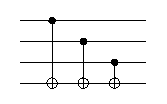
\includegraphics[scale=2]{Figures/circuits/proof1}};   
      \coordinate[below left=7mm and -6mm of c6.west] (l6);
      \coordinate[right=45mm of l6] (r6);
      \pic (cut6) {cut=l6/r6};  
    \end{tikzpicture}
  };
\end{tikzpicture}
\vspace*{140mm}
\caption{Proof of the implementation of multiple non-local CNOT gates that share a common target. The proof uses properties given in Figures~\ref{fig:props}, \ref{fig:sliding} and~\ref{fig:nonlocalCNOTs}. The distributed circuit is similar to the case for share control (Figure~\ref{fig:nonlocalCNOTs}). Both cat-entangler and cat-disentangler slightly differ.}
\label{fig:CNOTtargetProof}
\end{figure}

\section{Finding an efficient distribution}
\label{EfficientDistrib}

In this section we explain how we search for an efficient distribution of the circuit. First, we establish what we mean by a distributed circuit to be efficient. This notion is based on our discussion about the essential characteristics of distributed quantum architectures (see \S\ref{DQC_Architecture}). We say that a distributed circuit is efficient when there is:

\begin{itemize}
  \item \textit{Minimal amount of quantum communication} between the QPUs, meaning it requires as little number of ebits as possible. In comparison, message passing of classical bits is considered negligible and it is not taken into account.
  \item \textit{Load-balance across the QPUs}, up to a tolerance margin. Our notion of load-balance is that the different QPUs should have a similar number of qubits assigned to them. Uniform depth of the local circuits (i.e.\ length of the circuits) would also be desirable. However, none of our distribution techniques change the depth in a significant way. Hence, we will not optimise circuit depth when distributing a circuit, and instead assume that methods for depth reduction, such as the one described by~\citet{DepthReduction}, have already been applied on the input circuit, and may be applied again to each QPU's local circuit. As we do not take into account circuit depth, we consider the cost of local gates negligible.
\end{itemize}

The problem at hand is similar to the  \textit{(\(k,\varepsilon\))-graph partitioning} problem. In it, a graph partition in \(k\) subgraphs has to be found, minimising the number of \textit{cut edges}: edges that have their incident vertices in different subgraphs. Additionally, the partition must satisfy that the number of vertices in each subgraph is less than \((1 \pm \varepsilon)\frac{N}{k}\), where \(N\) is the total number of vertices in the graph. In Table~\ref{tab:matching} we list the correspondences between the graph partitioning problem and the efficient distribution of quantum circuits.

\begin{table}
\caption{Correspondence between the graph partitioning problem and the efficient distribution of quantum circuits.}
\label{tab:matching}
\centering
\begin{tabular}{|c|c|}
\hline
\textit{Graph partitioning} & \textit{Efficient distribution} \\
\hline
Vertices & Circuit wires (qubits) \\
Edges & CNOT gates \\
Partitioned graph & Distributed circuit \\
Subgraph & QPU \\
Min. cut edges & Min. non-local gates \\
Uniform subgraph size & Load-balance \\
\hline
\end{tabular}
\end{table}

But there is a caveat. If we use graph partitioning naively, we will not be exploiting the fact that multiple CNOT gates may be implemented using a single ebit. In what follows, we will explain how to make use of \textit{hypergraph} partitioning, to account for this aspect. A more detailed review of the hypergraph partition problem is given in Appendix~\ref{chap:HypPart}, here we summarise the key concepts:

\begin{itemize}
  \item Hypergraphs extend graphs to accommodate edges that may have more than two incident vertices. More formally, a hypergraph is a pair \((V,H)\), where \(V\) is the set of vertices and \(H \subseteq 2^V\) is the collection\footnote{We will allow the existence of multiple identical hyperedges, in the same way as multigraphs allow multiple edges across a pair of edges.} of hyperedges. Each hyperedge is defined as the subset of vertices from \(V\) it connects. We will not consider any notion of directionality.
  \item Hypergraph partitioning follows the same premise as graph partitioning. The user provides a hypergraph and two parameters \((k,\varepsilon)\), which have the exact same meaning as before. What the problem now attempts to minimise is a metric known as \(\lambda\!-\!1\), which is defined as follows: Given a partition of the hypergraph, the function \(\lambda\colon\, H \to \mathbb{N}\) maps each hyperedge to the number of different \textit{blocks}\footnote{The term \textit{block} is often used to refer to each of the sub-hypergraphs the hypergraph is partitioned into. It is the term we will use throughout this thesis.} its vertices are in. Then, \(\lambda\!-\!1 = \sum_{h \in H} \lambda(h) - 1\) provides a measure of not only how many hyperedges are cut but also how many blocks they are connecting\footnote{Simply minimising the number of cut hyperedges is also an often used approach, but it is not as useful for our problem.}.
\end{itemize}

In the following subsections, we explain how hypergraph partitioning can be used to find the most efficient distribution of a circuit. First, we only use the implementation of non-local gates described by~\citet{NonLocalCNOT}, reviewed in \S\ref{IntroDistributing}. Later on, we extend the algorithm to include the improvements we have proposed in \S\ref{NonLocalGates}.

\subsection{Vanilla algorithm}
\label{Vanilla}

The main challenge is how to use hyperedges to represent a collection of CNOT gates that, in case of being non-local, they could all be implemented using a single ebit. In this first version of the algorithm, we will group CNOTs together only if they share a common control wire and there are no other gates in between their connections to that wire. For every such a collection of CNOT gates, we will create \textit{a single hyperedge}. The hyperedge's vertices will correspond to the controlling wire and each of the different wires the CNOTs target. Algorithm~\ref{code:buildHypVanilla} receives a circuit as input and builds its hypergraph in this way. 

\begin{algorithm}[caption={Builds the hypergraph of a given circuit. \(H\) may contain multiple hyperedges connecting the same vertices. This algorithm runs in time \(O(g)\), where \(g\) is the number of gates in the input circuit.}, label={code:buildHypVanilla}]
input: circuit
output: (V,H)
begin
  V $\gets$ $\varnothing$
  H $\gets$ $\varnothing$
  hedge $\gets$ $\varnothing$
  foreach wire in circuit do
    V $\gets$ V $\cup$ {wire}
    hedge $\gets$ {wire}
    foreach gate in wire do
      if gate == CNOT and $controlOf$(gate) == wire then
        hedge $\gets$ hedge $\cup$ {$targetOf$(gate)}
      else
        H $\gets$ H $+$ {hedge}
        hedge $\gets$ {wire}
    H $\gets$ H $+$ {hedge}
end
\end{algorithm}

%Besides, it may be surprising that our hyperedges do not indicate which of the vertices is the control wire. That information is irrelevant at the partitioning level: each time a hyperedge is cut, we will require an ebit to implement the non-local gates, no matter which QPU the control wire is assigned to. Such information is only relevant when transforming the circuit into its distributed form, which is the next step of our algorithm. 

We then solve the hypergraph partitioning problem (see Appendix~\ref{chap:HypPart}) on the resulting hypergraph. Once a partition of the hypergraph is obtained, we map the partition back to the circuit, distributing it. The way the vertices are assigned in the blocks determines how the corresponding wires are allocated to the different QPUs. The \(\lambda-1\) metric of the partition indicates the number of ebits that will be necessary to implement all the non-local CNOT gates. The problem of finding the optimal partition for a hypergraph built by Algorithm~\ref{code:buildHypVanilla}, and the problem of efficiently\footnote{Where efficiency is assessed as discussed in the beginning of this section.} distributing a circuit are equivalent -- given any solution to one of them, we can compute a solution for the other. We formalise this fact in the Theorem~\ref{thm:vanilla}. 

Figures~\ref{fig:vanillaCutsA}, \ref{fig:vanillaCutsB} and~\ref{fig:vanillaCutsC} provide simple examples of the one-to-one correspondence discussed in Theorem~\ref{thm:vanilla}. In these figures, and in all of the figures throughout this thesis, hypergraphs are represented using the following convention: Letters are vertices, and each hyperedge is represented as a collection of line segments that reach each of the hyperedge's vertices, while the other end of the segments meet at the same point. A hypergraph partition is represented in a similar way as a partition of circuits; a dashed grey line splits the hypergraph, determining which vertices go to each block.

\textbf{TODO} Figure showing the different cases from the paragraph above, a and b. Give both the original circuit with dashed splits, the hypergraph and the black boxed distributed circuit (fig:vanillaCuts)
\begin{figure}
\centering
\begin{tikzpicture}
  \node (distributed) {
    \begin{tikzpicture}
      \node[inner sep=0pt] (circuit) {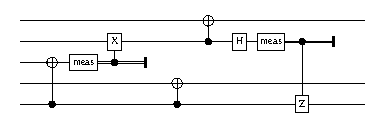
\includegraphics[scale=2]{Figures/circuits/vanillaCuts0}};
      \pic (e1) {ebit=e1/12.67mm/13mm};
      \coordinate[above left=3.6mm and -6mm of circuit.west] (leftPoint);
      \coordinate[above right=3.6mm and -6mm of circuit.east] (rightPoint);
      \pic (cut) {cut=leftPoint/rightPoint};
      \node[above left=11.5mm and -7mm of circuit.west, opacity=0.9] {\footnotesize \(A\)};
      \node[below left=4.5mm and -7mm of circuit.west, opacity=0.9] {\footnotesize \(B\)};
      \node[below left=11.5mm and -7mm of circuit.west, opacity=0.9] {\footnotesize \(C\)};
      \node[right=-3mm of circuit.north west, font=\itshape] (text) {c)};
    \end{tikzpicture}
  };
  \node[above left=-3mm and -70mm of distributed] (template) {
    \begin{tikzpicture}
      \node[inner sep=0pt] (circuit) {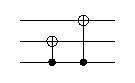
\includegraphics[scale=2]{Figures/circuits/vanillaCutsTemplate}};  
      \coordinate[above left=3.6mm and -6mm of circuit.west] (leftPoint);
      \coordinate[above right=3.6mm and -6mm of circuit.east] (rightPoint);
      \pic (cut) {cut=leftPoint/rightPoint};
      \node[above left=4.5mm and -7mm of circuit.west, opacity=0.9] {\footnotesize \(A\)};
      \node[left=-7mm of circuit.west, opacity=0.9] {\footnotesize \(B\)};
      \node[below left=4.5mm and -7mm of circuit.west, opacity=0.9] {\footnotesize \(C\)};
      \node[right=-3mm of circuit.north west, font=\itshape] (text) {a)};
    \end{tikzpicture}
  };
  \node[above right=-26.5mm and 10mm of template] (hypergraph) {
    \begin{tikzpicture}
      \coordinate (O) at (0,0);
      \coordinate (A) at (90:10mm);
      \coordinate (B) at (210:10mm);
      \coordinate (C) at (330:10mm);
      \draw (O) -- (A);
      \draw (O) -- (B);
      \draw (O) -- (C);
      \node[circle, right=-2.5mm of A, fill=white, inner sep=0pt, minimum size=5mm] {\(A\)};
      \node[circle, right=-2.5mm of B, fill=white, inner sep=0pt, minimum size=5mm] {\(B\)};
      \node[circle, right=-2.5mm of C, fill=white, inner sep=0pt, minimum size=5mm] {\(C\)};
      \coordinate[above left=5.3mm and 9mm of O] (leftPoint);
      \coordinate[above right=5.3mm and 9mm of O] (rightPoint);
      \pic (cut) {cut=leftPoint/rightPoint};
      \node[above left=0mm and 9mm of A, font=\itshape] (text) {b)};
    \end{tikzpicture}
  };
\end{tikzpicture}
\caption{The CNOTs in the circuit \textit{a)} are adjacent at their control wire. Therefore, a single hyperedge is used to represent both in \textit{b)}. The proposed cut makes only one of the CNOTs non-local, which is implemented in \textit{c)} using one ebit.}
\label{fig:vanillaCutsA}
\end{figure}

\begin{figure}
\centering
\begin{tikzpicture}
  \node (distributed) {
    \begin{tikzpicture}
      \node[inner sep=0pt] (circuit) {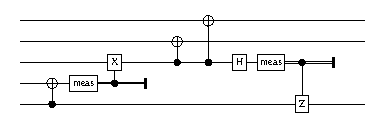
\includegraphics[scale=2]{Figures/circuits/vanillaCuts1}};
      \pic (e1) {ebit=e1/19.75mm/13mm};
      \coordinate[above left=-3.6mm and -6mm of circuit.west] (leftPoint);
      \coordinate[above right=-3.6mm and -6mm of circuit.east] (rightPoint);
      \pic (cut) {cut=leftPoint/rightPoint};
      \node[above left=11.5mm and -7mm of circuit.west, opacity=0.9] {\footnotesize \(A\)};
      \node[above left=4.5mm and -7mm of circuit.west, opacity=0.9] {\footnotesize \(B\)};
      \node[below left=11.5mm and -7mm of circuit.west, opacity=0.9] {\footnotesize \(C\)};
      \node[right=-3mm of circuit.north west, font=\itshape] (text) {c)};
    \end{tikzpicture}
  };
  \node[above left=-3mm and -70mm of distributed] (template) {
    \begin{tikzpicture}
      \node[inner sep=0pt] (circuit) {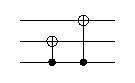
\includegraphics[scale=2]{Figures/circuits/vanillaCutsTemplate}};  
      \coordinate[below left=3.6mm and -6mm of circuit.west] (leftPoint);
      \coordinate[below right=3.6mm and -6mm of circuit.east] (rightPoint);
      \pic (cut) {cut=leftPoint/rightPoint};
      \node[above left=4.5mm and -7mm of circuit.west, opacity=0.9] {\footnotesize \(A\)};
      \node[left=-7mm of circuit.west, opacity=0.9] {\footnotesize \(B\)};
      \node[below left=4.5mm and -7mm of circuit.west, opacity=0.9] {\footnotesize \(C\)};
      \node[right=-3mm of circuit.north west, font=\itshape] (text) {a)};
    \end{tikzpicture}
  };
  \node[above right=-30mm and 10mm of template] (hypergraph) {
    \begin{tikzpicture}
      \coordinate (O) at (0,0);
      \coordinate (A) at (90:10mm);
      \coordinate (B) at (210:10mm);
      \coordinate (C) at (330:10mm);
      \draw (O) -- (A);
      \draw (O) -- (B);
      \draw (O) -- (C);
      \node[circle, right=-2.5mm of A, fill=white, inner sep=0pt, minimum size=5mm] {\(A\)};
      \node[circle, right=-2.5mm of B, fill=white, inner sep=0pt, minimum size=5mm] {\(B\)};
      \node[circle, right=-2.5mm of C, fill=white, inner sep=0pt, minimum size=5mm] {\(C\)};
      \coordinate (leftPoint) at (270:10.5mm);
      \coordinate (rightPoint) at (30:10.5mm);
      \pic (cut) {cut=leftPoint/rightPoint};
      \node[above left=0mm and 9mm of A, font=\itshape] (text) {b)};
    \end{tikzpicture}
  };
\end{tikzpicture}
\caption{Same as in Figure~\ref{fig:vanillaCutsA}, but now the cut makes both CNOTs non-local. Still, only one ebit is required, as implied by the hypergraph \textit{b)}. When CNOTs share their control wire, an ebit is required iff any of the target wires is in a different QPU than the control wire's QPU.}
\label{fig:vanillaCutsB}
\end{figure}

\begin{figure}
\hspace*{0mm}
\begin{tikzpicture}
  \node (template) {
    \begin{tikzpicture}
      \node[inner sep=0pt] (circuit) {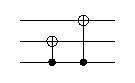
\includegraphics[scale=2]{Figures/circuits/vanillaCutsTemplate}};  
      \coordinate[below left=3.6mm and -6mm of circuit.west] (leftPoint1);
      \coordinate[below right=3.6mm and -6mm of circuit.east] (rightPoint1);
      \pic (cut1) {cut=leftPoint1/rightPoint1};
      \coordinate[above left=3.6mm and -6mm of circuit.west] (leftPoint2);
      \coordinate[above right=3.6mm and -6mm of circuit.east] (rightPoint2);
      \pic (cut2) {cut=leftPoint2/rightPoint2};
      \node[above left=4.5mm and -7mm of circuit.west, opacity=0.9] {\footnotesize \(A\)};
      \node[left=-7mm of circuit.west, opacity=0.9] {\footnotesize \(B\)};
      \node[below left=4.5mm and -7mm of circuit.west, opacity=0.9] {\footnotesize \(C\)};
      \node[right=-3mm of circuit.north west, font=\itshape] (text) {a)};
    \end{tikzpicture}
  };
  \node[above right=-28mm and 10mm of template] (hypergraph) {
    \begin{tikzpicture}
      \coordinate (O) at (0,0);
      \coordinate (A) at (90:10mm);
      \coordinate (B) at (210:10mm);
      \coordinate (C) at (330:10mm);
      \draw (O) -- (A);
      \draw (O) -- (B);
      \draw (O) -- (C);
      \node[circle, right=-2.5mm of A, fill=white, inner sep=0pt, minimum size=5mm] {\(A\)};
      \node[circle, right=-2.5mm of B, fill=white, inner sep=0pt, minimum size=5mm] {\(B\)};
      \node[circle, right=-2.5mm of C, fill=white, inner sep=0pt, minimum size=5mm] {\(C\)};
      \coordinate[above left=5.3mm and 9mm of O] (leftPoint);
      \coordinate[above right=5.3mm and 9mm of O] (rightPoint);
      \pic (cut) {cut=leftPoint/rightPoint};
      \coordinate (leftPoint2) at (270:10.5mm);
      \coordinate (rightPoint2) at (30:10.5mm);
      \pic (cut2) {cut=leftPoint2/rightPoint2};
      \coordinate (extraPoint) at (30:16mm);
      \pic (cut3) {cut=rightPoint2/extraPoint};
      \node[above left=0mm and 9mm of A, font=\itshape] (text) {b)};
    \end{tikzpicture}
  };
  \node[below right=2mm and -73mm of template] (distributed) {
    \begin{tikzpicture}[transform canvas={scale=0.65}]
      \node[inner sep=0pt] (circuit) {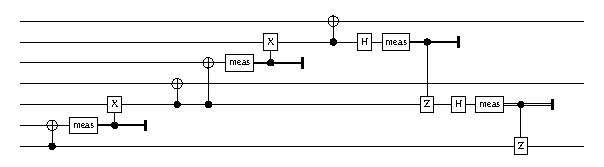
\includegraphics[scale=2]{Figures/circuits/vanillaCuts2}};
      \pic (e1) {ebit=e1/12.67mm/13mm};
      \pic (e2) {ebit=e2/33.84mm/13mm};
      \coordinate[above left=10.6mm and -6mm of circuit.west] (leftPoint);
      \coordinate[above right=10.6mm and -6mm of circuit.east] (rightPoint);
      \pic (cut) {cut=leftPoint/rightPoint};
      \coordinate[below left=10.6mm and -6mm of circuit.west] (leftPoint2);
      \coordinate[below right=10.6mm and -6mm of circuit.east] (rightPoint2);
      \pic (cut2) {cut=leftPoint2/rightPoint2};
      \node[above left=18.5mm and -7mm of circuit.west, opacity=0.9] {\footnotesize \(A\)};
      \node[left=-7mm of circuit.west, opacity=0.9] {\footnotesize \(B\)};
      \node[below left=18.5mm and -7mm of circuit.west, opacity=0.9] {\footnotesize \(C\)};
    \end{tikzpicture}
  };
  \node[right=-3mm of distributed.north west, font=\itshape] (text) {c)};
\end{tikzpicture}
\vspace*{38mm}
\caption{Same as in Figure~\ref{fig:vanillaCutsA}, but now there are two cuts, distributing the circuit across three QPUs.}
\label{fig:vanillaCutsC}
\end{figure}

\begin{theorem} Given any circuit \(\mathcal{C}\), and its hypergraph \(\mathcal{H}\) generated by Algorithm~\ref{code:buildHypVanilla}, there is a bijection between partitions of \(\mathcal{H}\) with \(\lambda_c\) cuts and vanilla\footnote{Meaning that non-local CNOT gates may only be implemented using the remote-control method from Figure~\ref{fig:nonlocalCNOTs}.} distributions of \(\mathcal{C}\) that use \(\lambda_e\) ebits.
\label{thm:vanilla}
\end{theorem} \begin{proof}
We define this bijection inductively. First, we provide the bijection between the \textit{trivial configurations}:
\begin{itemize}
  \item The partition of \(\mathcal{H}\) where all vertices are in the same block corresponds one-to-one to 
  \item the whole circuit \(\mathcal{C}\) being executed in a single QPU.
\end{itemize}

Then, we define a \textit{primitive transformation} for both problems, which allows us to move vertices/wires around. To do so, we use the one-to-one correspondence between vertices and wires that Algorithm~\ref{code:buildHypVanilla} imposes. We additionally require to have an indexed set of hypergraph blocks and QPUs.
\begin{itemize}
  \item Given a partition of \(\mathcal{H}\), moving vertex \(x\) from block \(i\) to block \(j\) corresponds one-to-one to
  \item picking wire \(x\) -- which is guaranteed to be in QPU \(i\) -- and allocating it in QPU \(j\).
\end{itemize}

Using this primitive, any partition/distribution can be reached, so we indeed have a bijection. Notice that wire \(x\) was guaranteed to be in QPU \(i\) thanks to our inductive definition of the bijection itself: all vertices/wires start in the same block (trivial configuration), while the primitive moves any \(x\) vertex/wire respectively to a block or a QPU, both indexed by the same \(j\). It remains to prove that the given bijection preserves the match between the number of cuts \(\lambda_c\) and the number of ebits \(\lambda_e\). We give a proof by induction over the sequence of primitives that, starting from the trivial configuration, generates the partition/distribution.

\begin{itemize}
  \item The trivial configuration of both problems has \(\lambda_c = 0 = \lambda_e\).
  \item Given a sequence of \(n+1\) primitives, we assume that \(\lambda_c = \lambda_e\) holds after the \(n\)-th primitive was applied (our induction hypothesis). We must prove that it still holds after the \((n+1)\)-th primitive is applied. When a vertex is reallocated, all of its hyperedges are affected, which may create/remove multiple cuts. We will consider the contribution of each of these hyperedges separately. Besides, reallocating vertex \(x\) from block \(i\) to block \(j\), as determined by the \((n+1)\)-th primitive, may affect each hyperedge \(h\) differently whether \(x\) corresponds to the control wire shared by all the CNOTs represented in \(h\), or it corresponds to a target wire. If \(x\) corresponds to a target wire, applying the primitive may:
    \begin{enumerate}
    \renewcommand{\theenumi}{\alph{enumi})}
      \item \textit{Increase} \(\lambda_c\). \(\lambda_c\) increases by one iff a new cut is added to the hyperedge \(h\). This happens iff the block/QPU \(j\) did not already contain a vertex/wire from \(h\). In that case, \(x\) becomes an isolated target wire, and to implement its CNOT it will be necessary and sufficient to create an extra ebit, increasing \(\lambda_e\) by one. Therefore, \(\lambda_e\) will increase iff \(\lambda_c\) does so, both by the same amount.
      \item \textit{Decrease} \(\lambda_c\). In the same spirit, \(\lambda_c\) decreases by one iff a previously isolated target vertex/wire is allocated where some fellow vertices/wires are. When and only when this happens, one less ebit will be required, as the previously isolated target wire \(x\) will no longer need its own ebit: it will either use an existent one or be allocated to the same QPU as the control wire. Therefore, \(\lambda_e\) will decrease iff \(\lambda_c\) does so, both by the same amount.
    \end{enumerate}
\end{itemize}

When \(x\) is the control wire of the CNOTs in \(h\), we analyse the reallocation of \(x\) from \(i\) to \(j\) as a multiple step process. First, we will relabel block/QPU \(i\) as \(j\) and vice versa. Evidently, this does not change either \(\lambda_c\) or \(\lambda_e\). Then, we reallocate each of the other vertices from \(h\) that were affected by this relabelling -- all corresponding to target wires -- back to their block/QPU. Thus, the effect on \(\lambda_c\) and \(\lambda_e\) is completely described by the two cases listed above.

Therefore, starting from \(\lambda_c = \lambda_e = 0\), and applying the whole sequence of primitives one by one, maintains \(\lambda_c = \lambda_e\).

\end{proof}

\begin{comment}
\begin{algorithm}[caption={Builds the distributed circuit determined by the input hypergraph partition. The hypergraph partition is provided as an assignment \(qpuOf \colon \mathbb{N} \to \mathbb{N}\) which indicates the QPU number of the given wire},label={code:distributeVanilla}]
input: circuit, $qpuOf$
output: distributed
begin
  distributed $\gets$ $emptyCircuit$
  foreach wire in circuit do
    thisQPU = $qpuOf$(wire)
    activeConnections $\gets$ $\varnothing$
    foreach gate in wire do
      if gate == CNOT and $controlOf$(gate) == wire then
        targetQPU = $qpuOf$($targetOf$(gate))
        if targetQPU == thisQPU then
          distributed.$addCNOTAt$(wire,target)
        else
          ebit $\gets$ activeConnections.$at$(targetQPU)
          if ebit == null then
            ebit $\gets$ $distillEbit$(thisQPU, targetQPU)
            distributed.$addCatEntangler$(ebit, wire)
            activeConnections.$at$(targetQPU) $\gets$ ebit
          distributed.$addCNOTAt$(ebit,$targetOf$(gate))
      else
        distributed.$addGateAt$(gate,wire)
end
\end{algorithm}
\end{comment}

% Algorithm~\ref{code:distributeVanilla} performs the transformation from hypergraph partition to distributed circuit. Notice that this algorithm may alter the ordering of some of the gates, as a CNOT gate could be inserted before the previous gates on its target wire have been added. Some bookmarking must be kept to prevent this, but the details are straight-forward

\begin{remark} \normalfont 
In Figure~\ref{fig:vanillaCutsC}, the second cat-entangler `copies' the information held by the local ebit half previously entangled with wire \(C\), instead of being directly coupled with with \(C\). The latter option would also be correct\footnote{However, in that case, wires \(B\) and \(C\) should interchange places in the circuit representation if we want to visualise in 2D that only ebits and classical information crosses the boundary between QPUs.}. Either of these ways is represented by the same hypergraph partition, so in order to maintain our one-to-one correspondence, we should rather say there is a bijection between hypergraph partitions and equivalence classes\footnote{Families of circuit distributions that are equivalent in the sense that their wires are allocated to the same way, and that the number of ebits required also matches.} of circuit distributions. Although for our algorithm all of the solutions in one such equivalence class are indistinguishable, some of the solutions will offer a more decentralised network of ebits than others. Optimisations taking this fact into account could be performed as post-processing of our proposed algorithm.
\end{remark}

A closer look at the bijection proposed in Theorem~\ref{thm:vanilla} reveals that we can transform back and forth between hypergraph partition and circuit distribution in polynomial time: To go from partition to distribution, we just need to read where each of the vertices are assigned, and apply the primitive to move each wire to its QPU -- which affects all the CNOTs on that wire. The opposite direction works the same way. Hence, the time complexity of the transformation in either direction is \(O(n\cdot m)\), where \(n\) is the number of vertices/wires and \(m\) the number of hyperedges/CNOTs. This leads us to two results, one per direction of the bijection:

\begin{corollary} The best vanilla distribution of a circuit can be efficiently derived from an optimal partition of the hypergraph built by Algorithm~\ref{code:buildHypVanilla}.
\label{col:vanilla}
\end{corollary} \begin{proof}
We know it will be the best distribution thanks to Theorem~\ref{thm:vanilla}: The optimal partition will have the lowest possible \(\lambda_c\), and given that at any point \(\lambda_c = \lambda_e\), the corresponding circuit distribution will also have the lowest \(\lambda_e\) possible.

We say the circuit distribution is efficiently derived because the required transformations -- Algorithm~\ref{code:buildHypVanilla} and the translation from hypergraph partition to circuit distribution -- both run in polynomial time.

\end{proof}

\begin{corollary} The quantum circuit distribution problem is an NP-complete problem.
\label{col:np}
\end{corollary} \begin{proof}
To prove NP-completeness we simply need to show that, in case the quantum circuit distribution problem could be solved in polynomial time, we would be able to solve an NP-complete problem in polynomial time. The hypergraph partitioning problem happens to be NP-complete \citep{NP-complete}, and Theorem~\ref{thm:vanilla} allows us to take the solution for the circuit efficient distribution problem and provide the optimal partition of its hypergraph. The only caveat is that we need to be able to do this for any hypergraph \(\mathcal{H}\), so we must be able to build a non-distributed circuit \(\mathcal{C}\) that is represented by \(\mathcal{H}\) -- the opposite direction of what Algorithm~\ref{code:buildHypVanilla} does. There will be multiple such circuits; building one of these in polynomial time is possible, and the details are straight-forward.

\end{proof}

On the pessimistic side, Corollary~\ref{col:np} means that unless \(P=NP\), finding the best distribution of an arbitrary quantum circuit takes exponential time. On the optimistic side, many problems that compilers from classical computer science deal with are also NP-complete. In order to implement fast compilers that prepare quantum algorithms to be run in distributed architectures, we will not need to design better algorithms to solve our particular problem: we may use the already rich research on fast algorithms for hypergraph partitioning \citep{KaHyPart}, as the polynomial overhead of transforming back and forth between problems will be negligible.


\begin{figure}
\hspace*{0mm}
\begin{tikzpicture}
  \node (template) {
    \begin{tikzpicture}
      \node[inner sep=0pt] (circuit) {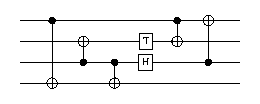
\includegraphics[scale=2]{Figures/circuits/vanillaCirc}};  
      \node[above left=8mm and -7mm of circuit.west, opacity=0.9] {\footnotesize \(A\)};
      \node[above left=1mm and -7mm of circuit.west, opacity=0.9] {\footnotesize \(B\)};
      \node[below left=1mm and -7mm of circuit.west, opacity=0.9] {\footnotesize \(C\)};
      \node[below left=8mm and -7mm of circuit.west, opacity=0.9] {\footnotesize \(D\)};
      \node[right=-3mm of circuit.north west, font=\itshape] (text) {a)};
    \end{tikzpicture}
  };
  \node[above right=-35.5mm and 6mm of template] (hypergraph) {
    \begin{tikzpicture}
      \coordinate (O) at (0,0);
      \coordinate (B) at (45:13mm);
      \coordinate (A) at (135:13mm);
      \coordinate (C) at (225:13mm);
      \coordinate (D) at (315:13mm);
      \coordinate (auxB) at (45:4.5mm);
      \coordinate (auxD) at (315:4.5mm);
      \draw (A) -- (C);
      \draw (A) -- (auxB);
      \draw (B) -- (auxB);
      \draw (D) -- (auxB);
      \draw (C) -- (auxD);
      \draw (B) -- (auxD);
      \draw (D) -- (auxD);
      \node[circle, right=-2.5mm of A, fill=white, inner sep=0pt, minimum size=5mm] {\(A\)};
      \node[circle, right=-2.5mm of B, fill=white, inner sep=0pt, minimum size=5mm] {\(B\)};
      \node[circle, right=-2.5mm of C, fill=white, inner sep=0pt, minimum size=5mm] {\(C\)};
      \node[circle, right=-2.5mm of D, fill=white, inner sep=0pt, minimum size=5mm] {\(D\)};
      \coordinate[above left=9mm and 1mm of O] (leftPoint);
      \coordinate[below left=9mm and 1mm of O] (rightPoint);
      \pic (cut) {cut=leftPoint/rightPoint};
      \node[above left=5mm and 9mm of A, font=\itshape] (text) {b)};
    \end{tikzpicture}
  };
  \node[below right=4mm and -92mm of template] (distributed) {
    \begin{tikzpicture}[transform canvas={scale=0.58}]
      \node[inner sep=0pt] (circuit) {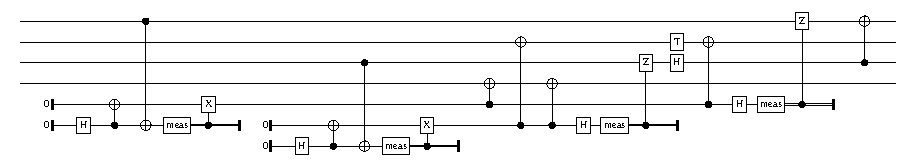
\includegraphics[scale=2]{Figures/circuits/vanillaDistrib}};
      \pic (e2) {ebitLong=e2/19.76mm/15.5mm};
      \pic (e1) {ebitLessClear=e1/26.8mm/16mm};
      \coordinate[left=-4mm of circuit.west] (leftPoint);
      \coordinate[right=-4mm of circuit.east] (rightPoint);
      \pic (cut) {cut=leftPoint/rightPoint};
      \node[above left=22mm and -7mm of circuit.west, opacity=0.9] {\(B\)};
      \node[above left=15mm and -7mm of circuit.west, opacity=0.9] {\(D\)};
      \node[below left=15mm and -7mm of circuit.west, opacity=0.9] {\(A\)};
      \node[below left=22mm and -7mm of circuit.west, opacity=0.9] {\(C\)};
    \end{tikzpicture}
  };
  \node[right=-1mm of distributed.north west, font=\itshape] (text) {c)};
\end{tikzpicture}
\vspace*{38mm}
\caption{The circuit is distributed using only \(2\) ebits. The other two possible distributions: \(\{\{A,B\},\{C,D\}\}\) and \(\{\{A,D\},\{B,C\}\}\) both require \(3\) ebits to be implemented. The wires in the distributed version of the circuit have been rearranged, so it is possible to visualise in a planar diagram that no quantum information crosses the boundary.}
\label{fig:vanillaExample}
\end{figure}


A simple circuit, its optimally partitioned hypergraph and the resulting distributed circuit are shown in Figure~\ref{fig:vanillaExample}. Each of the QPUs can be set to implement its own local circuit, distilling ebits and using them along classical communication when indicated.


\subsection{\texttt{SlideCNOTs}: Bringing CNOT gates together}
\label{pullCNOTs}


\footnotetext{Even though in a distributed circuit no quantum information crosses the QPU boundary (apart from the shared ebits), not every distributed circuit can be visualised in 2D in a way that no CNOT crosses it. In graph theory this is known as the \textit{planarity} problem.}

In Figure~\ref{fig:pullRules} we showed that any 1-qubit gate in the Clifford+T set acting on the control wire of a CNOT gate, with the exception of the H gate, can commute with the CNOT up to some byproduct. Here we use this fact, applying some pre-processing on the input circuit that brings together nearby CNOT gates, allowing us to implement more non-local CNOTs using a single ebit. Figure~\ref{fig:pulledCNOTexample} gives an example of how these transformations -- listed in Figure~\ref{fig:pullRules} -- can lead to a more efficient distribution of the circuit. We will refer to the pre-processing described in this subsection as \texttt{SlideCNOTs}.

\begin{figure}
\centering
\begin{tikzpicture}
  \node (circ) {
    \begin{tikzpicture}
      \node[inner sep=0pt] (circuit) {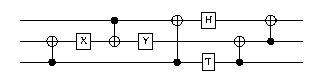
\includegraphics[scale=2, trim={2.5mm 0 2.5mm 0}, clip]{Figures/circuits/pullCirc}};  
      \node[left=-7mm of circuit.west, rectangle,fill=white,minimum height=22mm, minimum width=8mm] {};
      \node[right=-7mm of circuit.east, rectangle,fill=white,minimum height=22mm, minimum width=8mm] {};
      \node[above left=4.5mm and -7mm of circuit.west, opacity=0.9] {\footnotesize \(A\)};
      \node[left=-7mm of circuit.west, opacity=0.9] {\footnotesize \(B\)};
      \node[below left=4.5mm and -7mm of circuit.west, opacity=0.9] {\footnotesize \(C\)};
      \node[right=-3mm of circuit.north west, font=\itshape] (text) {a)};
    \end{tikzpicture}
  };
  \node[below=5mm of circ] (pulled) {
    \begin{tikzpicture}
      \node[inner sep=0pt] (circuit) {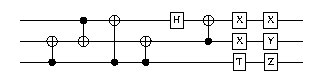
\includegraphics[scale=2, trim={2.5mm 0 2.5mm 0}, clip]{Figures/circuits/pullPulled}};  
      \node[left=-7mm of circuit.west, rectangle,fill=white,minimum height=22mm, minimum width=8mm] {};
      \node[right=-7mm of circuit.east, rectangle,fill=white,minimum height=22mm, minimum width=8mm] {};
      \node[above left=4.5mm and -7mm of circuit.west, opacity=0.9] {\footnotesize \(A\)};
      \node[left=-7mm of circuit.west, opacity=0.9] {\footnotesize \(B\)};
      \node[below left=4.5mm and -7mm of circuit.west, opacity=0.9] {\footnotesize \(C\)};
      \node[right=-3mm of circuit.north west, font=\itshape] (text) {c)};
    \end{tikzpicture}
  };
  \node[above right=-32.5mm and -2mm of circ] (hypergraph) {
    \begin{tikzpicture}
      \coordinate (O) at (0,0);
      \coordinate (A) at (90:12mm);
      \coordinate (B) at (210:12mm);
      \coordinate (C) at (330:12mm);
      \draw (O) -- (A);
      \draw (O) -- (B);
      \draw (O) -- (C);
      \draw (A) edge[out=210,in=90,looseness=1] (B); 
      \draw (A) -- (B);
      \draw (B) -- (C);
      \node[circle, right=-2.5mm of A, fill=white, inner sep=0pt, minimum size=5mm] {\(A\)};
      \node[circle, right=-2.5mm of B, fill=white, inner sep=0pt, minimum size=5mm] {\(B\)};
      \node[circle, right=-2.5mm of C, fill=white, inner sep=0pt, minimum size=5mm] {\(C\)};
      \coordinate (leftPoint) at (270:11.5mm);
      \coordinate (rightPoint) at (30:11.5mm);
      \pic (cut) {cut=leftPoint/rightPoint};
      \node[above left=0mm and 13mm of A, font=\itshape] (text) {b)};
    \end{tikzpicture}
  };
  \node[above right=-32.5mm and -2mm of pulled] (hypergraph2) {
    \begin{tikzpicture}
      \coordinate (O) at (0,0);
      \coordinate (A) at (90:12mm);
      \coordinate (B) at (210:12mm);
      \coordinate (C) at (330:12mm);
      \draw (O) -- (A);
      \draw (O) -- (B);
      \draw (O) -- (C);
      \draw (A) edge[out=210,in=90,looseness=1] (B); 
      \draw (A) -- (B);
      \node[circle, right=-2.5mm of A, fill=white, inner sep=0pt, minimum size=5mm] {\(A\)};
      \node[circle, right=-2.5mm of B, fill=white, inner sep=0pt, minimum size=5mm] {\(B\)};
      \node[circle, right=-2.5mm of C, fill=white, inner sep=0pt, minimum size=5mm] {\(C\)};
      \coordinate (leftPoint) at (270:11.5mm);
      \coordinate (rightPoint) at (30:11.5mm);
      \pic (cut) {cut=leftPoint/rightPoint};
      \node[above left=0mm and 13mm of A, font=\itshape] (text) {d)};
    \end{tikzpicture}
  };
\end{tikzpicture}
\vspace*{5mm}
\caption{Example where an ebit can be saved by sliding CNOTs closer together. This figure shows the original circuit \textit{a)}, its optimally partitioned hypergraph \textit{b)}, the pre-processed circuit \textit{c)}, and its optimally partitioned hypergraph \textit{d)}, which has one less cut hyperedge.}
\label{fig:pulledCNOTexample}
\end{figure}

The procedure is fairly straight-forward: Exploring the circuit from left to right, whenever a CNOT gate is found, use the transformations listed in Figure~\ref{fig:pullRules} to move it as early in the circuit as possible. The procedure introduces some additional \(X\) and \(Z\) gates. Fortunately, \(X\) and \(Z\) are their own inverse (i.e.\ \(XX = I\) and \(ZZ = I\)) and every 1-qubit gate in Clifford+T can be interchanged with \(X\) and \(Z\) in a simple way (as shown in Figure~\ref{fig:props}). Hence, we should expect no significant increase in the depth (i.e.\ length) of the circuit, as most byproduct gates will cancel each other out.

So far we have been talking about standard 1-qubit gates, but in practical circuits we are likely to find 1-qubit gates that are \textit{classically controlled}, meaning that a classical signal (a bit, either \(0\) or \(1\)) decides whether the gate is applied or not. These gates are commonly used to perform corrections on qubits after a measurement is done during the computation. These classically controlled gates are no issue for the distribution of the circuit, as the classical control may only require classical communication between QPUs. Concerning the pre-processing we just described, classically controlled 1-qubit gates can commute with CNOT under the exact same circumstances as their uncontrolled version. The only difference is that, whenever a byproduct gate is created, we must make sure it is controlled by the same classical signal that controlled the original gate, as shown in Figure~\ref{fig:classicalControl}.

\begin{figure}
\centering
\begin{tikzpicture}
  \node {
    \begin{tikzpicture}
      \node[inner sep=0pt] (circuit) at (0,0) {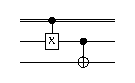
\includegraphics[scale=2]{Figures/circuits/classicalControl}};
      \node[right=0mm of circuit.north west, font=\itshape] (text) {a)};
    \end{tikzpicture}
    \hspace{8mm}
    \begin{tikzpicture}
      \node[inner sep=0pt] (circuit) at (0,0) {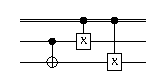
\includegraphics[scale=2]{Figures/circuits/classicalControl2}};
      \node[right=0mm of circuit.north west, font=\itshape] (text) {b)};
    \end{tikzpicture}
  };
\end{tikzpicture}
\caption{Pushing a classically controlled gate through a CNOT. The same rule as in Figure~\ref{fig:pullRules} is applied, while making sure any new gate is also controlled. Here, only the case for \(X\) gate is shown, but this works for any of the transformations in Figure~\ref{fig:pullRules}.}
\label{fig:classicalControl}
\end{figure}

The same procedure can be used to commute 1-qubit gates (except \(H\), \(S\) and \(T\)) across the target wire of the CNOT gates. This additional pre-processing would have no effect at all on the vanilla version of the algorithm, but it will be advantageous after we apply our next extension (\texttt{EitherRemote}), which benefits from CNOT gates to be adjacent on the target wire.

\begin{remark} 
Using \texttt{SlideCNOTs} will never increase the ebit count required to implement a partition.

\normalfont
This pre-processing simply moves the CNOTs along their wires. The same CNOTs that were non-local before \texttt{SlideCNOTs} was applied will still be non-local. On the worst case, these non-local CNOTs could be implemented in the exact same way as they were before, so the ebit count would remain the same.

\label{thm:SlideCNOTsImprove}
\end{remark}

\subsection{\texttt{EitherRemote}: Including the remote-target method}
\label{BothEnds}

In \S\ref{NonLocalGates} we showed that the trick for implementing multiple CNOT gates using a single ebit also works if they share a common target wire (instead of a control wire). This makes our optimisation problem more intricate: Now, when the CNOTs are to be implemented non-locally, we can choose to implement them using the remote-control or remote-target method. For explanation purposes, we will use two different kinds of hyperedges in this subsection's figures, depending on whether their CNOTs are controlled by the same wire, or act on the same target (thicker line). We will refer to the extension we propose in this subsection as \texttt{EitherRemote}.

\begin{figure}
\centering
\begin{tikzpicture}
  \node (circ) {
    \begin{tikzpicture}
      \node[inner sep=0pt] (circuit) {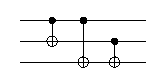
\includegraphics[scale=2]{Figures/circuits/bothEndsSimple}};  
      \node[above left=4.5mm and -7mm of circuit.west, opacity=0.9] {\footnotesize \(A\)};
      \node[left=-7mm of circuit.west, opacity=0.9] {\footnotesize \(B\)};
      \node[below left=4.5mm and -7mm of circuit.west, opacity=0.9] {\footnotesize \(C\)};
      \node[above right=0.8mm and 12.8mm of circuit.west, opacity=0.9] {\footnotesize \(\gamma\)};
      \node[below right=0.8mm and 23.6mm of circuit.west, opacity=0.9] {\footnotesize \(\beta\)};
      \node[below right=0.8mm and 34.4mm of circuit.west, opacity=0.9] {\footnotesize \(\alpha\)};
      \node[right=-3mm of circuit.north west, font=\itshape] (text) {a)};
    \end{tikzpicture}
  };
  \node[above right=-27mm and 5mm of circ] (controlHyp) {
    \begin{tikzpicture}
      \coordinate (O) at (0,0);
      \coordinate (A) at (90:10mm);
      \coordinate (B) at (210:10mm);
      \coordinate (C) at (330:10mm);
      \draw (O) -- (A);
      \draw (O) -- (B);
      \draw (O) -- (C);
      \draw (B) -- (C);
      \node[circle, right=-2.5mm of A, fill=white, inner sep=0pt, minimum size=5mm] {\(A\)};
      \node[circle, right=-2.5mm of B, fill=white, inner sep=0pt, minimum size=5mm] {\(B\)};
      \node[circle, right=-2.5mm of C, fill=white, inner sep=0pt, minimum size=5mm] {\(C\)};
      \node[above left=0mm and 13mm of A, font=\itshape] (text) {b)};
    \end{tikzpicture}
  };
  \node[right=-27mm and 15mm of circ] (targetHyp) {
    \begin{tikzpicture}
      \coordinate (O) at (0,0);
      \coordinate (A) at (90:10mm);
      \coordinate (B) at (210:10mm);
      \coordinate (C) at (330:10mm);
      \draw[ultra thick] (O) -- (A);
      \draw[ultra thick] (O) -- (B);
      \draw[ultra thick] (O) -- (C);
      \draw[ultra thick] (A) -- (B);
      \node[circle, right=-2.5mm of A, fill=white, inner sep=0pt, minimum size=5mm] {\(A\)};
      \node[circle, right=-2.5mm of B, fill=white, inner sep=0pt, minimum size=5mm] {\(B\)};
      \node[circle, right=-2.5mm of C, fill=white, inner sep=0pt, minimum size=5mm] {\(C\)};
      \node[above left=0mm and 13mm of A, font=\itshape] (text) {c)};
    \end{tikzpicture}
  };
  \node[below right=0mm and 0mm of circ] (bothHyp) {
    \begin{tikzpicture}
      \coordinate (O) at (0,0);
      \coordinate (auxC) at (4mm,3mm);
      \coordinate (auxT) at (-4mm,3mm);
      \coordinate (A) at (90:20mm);
      \coordinate (B) at (210:20mm);
      \coordinate (C) at (330:20mm);
      \draw[ultra thick] (auxT) -- (A);
      \draw[ultra thick] (auxT) -- (B);
      \draw[ultra thick] (auxT) -- (C);
      \draw[ultra thick] (A) -- (B);
      \draw (auxC) -- (A);
      \draw (auxC) -- (B);
      \draw (auxC) -- (C);
      \draw (B) -- (C);
      \node[circle, right=-2.5mm of A, fill=white, inner sep=0pt, minimum size=5mm] {\(A\)};
      \node[circle, right=-2.5mm of B, fill=white, inner sep=0pt, minimum size=5mm] {\(B\)};
      \node[circle, right=-2.5mm of C, fill=white, inner sep=0pt, minimum size=5mm] {\(C\)};
      \node[above left=0mm and 13mm of A, font=\itshape] (text) {c)};
    \end{tikzpicture}
  };
  \node[right=5mm of bothHyp] (hypergraph) {
    \begin{tikzpicture}
      \coordinate (O) at (0,0);
      \coordinate (auxA) at (90:9mm);
      \coordinate (auxC) at (330:9mm);
      \coordinate (A) at (90:18mm);
      \coordinate (B) at (210:18mm);
      \coordinate (C) at (330:18mm);
      \coordinate (a) at (270:9mm);
      \coordinate (b) at (30:9mm);
      \coordinate (c) at (150:9mm);
      \draw (auxA) -- (A);
      \draw (auxA) -- (b);
      \draw (auxA) -- (c);
      \draw[ultra thick] (auxC) -- (C);
      \draw[ultra thick] (auxC) -- (b);
      \draw[ultra thick] (auxC) -- (a);
      \draw (B) -- (a);
      \draw[ultra thick] (B) -- (c);
      \node[circle, right=-2.5mm of A, fill=white, inner sep=0pt, minimum size=5mm] {\(A\)};
      \node[circle, right=-2.5mm of B, fill=white, inner sep=0pt, minimum size=5mm] {\(B\)};
      \node[circle, right=-2.5mm of C, fill=white, inner sep=0pt, minimum size=5mm] {\(C\)};
      \node[circle, right=-2.5mm of a, fill=white, inner sep=0pt, minimum size=5mm] {\(\alpha\)};
      \node[circle, right=-2.5mm of b, fill=white, inner sep=0pt, minimum size=5mm] {\(\beta\)};
      \node[circle, right=-2.5mm of c, fill=white, inner sep=0pt, minimum size=5mm] {\(\gamma\)};
      \node[above left=0mm and 13mm of A, font=\itshape] (text) {e)};
    \end{tikzpicture}
  };
\end{tikzpicture}
\vspace*{5mm}
\caption{}
\label{fig:BothEndsChallenge}
\end{figure}

\textbf{TODO}: If the partition is \(\{\{A\},\{B,C\}\}\), then \(\alpha\) is a local CNOT, while \(\beta\) and \(\gamma\) are implemented using the common-control method. We know the common-control method must be used because the hyperedge cut is of the control type or, equivalently, because both \(\beta\) and \(\gamma\) vertices are assigned to the same block as their targets \(C\) and \(B\). Different line format for the hyperedges whether control or target.

\textbf{TODO}: Show cut that is best for common-target

\textbf{TODO}: Figure of hypergraphs from prev Fig; with control hyps, target hyps, naively. The dashed lines represent two hypothetical ways of partitioning the hypergraph. Different line format for the hyperedges whether control or target (fig:BothEndsChallenge)

Figure~\ref{fig:BothEndsChallenge} shows an example where using both the remote-control and remote-target methods in the same circuit is advantageous: CNOTs \(\alpha\) and \(\beta\) can be implemented using a single ebit if the remote-control method is used. CNOT \(\gamma\) is local, and CNOTs \(\delta\) and \(\eta\) can be implemented using a single ebit if the remote-target method is used. Therefore, we could distribute the circuit using only two ebits. However hypergraph \textit{b)}, built by Algorithm~\ref{code:buildHypVanilla}, can only be partitioned cutting at least three hyperedges. This is because, in hypergraph \textit{b)}, CNOTs are only grouped by common control, in `control-hyperedges' (thin lines). Hence, \(\delta\) and \(\eta\) appear as two distinct hyperedges: \(\{B,C\}\) and \(\{B,D\}\) respectively. Hypergraph \textit{c)} is the counterpart of \textit{b)} where `target-hyperedges' (thick lines) are used instead (i.e.\ CNOTs are grouped by common target). In this case, the minimum number of cuts is also three, as now it is \(\alpha\) and \(\beta\) the CNOTs that are not grouped together. Hypergraph \textit{d)} is a hybrid between the previous two, that can be partitioned cutting only two hyperedges. This is the hypergraph representation we will develop and use for the \texttt{EitherRemote} extension.

If we want to guarantee that a hypergraph partitioner can always find the most efficient circuit distribution, our hypergraph representation must have the following requirements:
\begin{enumerate}
  \item Both options of how to implement each non-local CNOT (remote-control and remote-target) are represented.
  \item A partition of the hypergraph must determine, for each non-local CNOT, which method should be used to implement it.
  \item The \(\lambda\!-\!1\) metric of a partition -- the number of cuts -- should accurately determine how many ebits are required to implement the circuit distribution it describes.
\end{enumerate}

\begin{algorithm}[caption={Builds the hypergraph of a given circuit, without choosing whether non-local CNOTs are implemented using the remote-control or the remote-target method. This algorithm runs in time \(O(g)\), where \(g\) is the number of gates in the input circuit.}, label={code:buildHypBothEnds}]
input: circuit
output: (V,H)
begin
  V $\gets$ $\varnothing$
  H $\gets$ $\varnothing$
  hedge $\gets$ $\varnothing$
  foreach wire in circuit do
    V $\gets$ V $\cup$ {wire}
    hedge $\gets$ {wire}
    hType $\gets$ $unknown$
    foreach gate in wire do
      if gate == CNOT then
        V $\gets$ V $\cup$ {$labelOf$(gate)}
        if $controlOf$(gate) == wire then
          if hType == $target$ then
            H $\gets$ H $+$ {hedge}
            hedge $\gets$ {wire}
          hType $\gets$ $control$
        if $targetOf$(gate) == wire then
          if hType == $control$ then
            H $\gets$ H $+$ {hedge}
            hedge $\gets$ {wire}  
          hType $\gets$ $target$
        hedge $\gets$ hedge $\cup$ {$labelOf$(gate)}
      else
        H $\gets$ H $+$ {hedge}
        hedge $\gets$ {wire}
        hType $\gets$ $unknown$
    H $\gets$ H $+$ {hedge}
end
\end{algorithm}

\begin{figure}
\centering
\begin{tikzpicture}
  \node (circ) {
    \begin{tikzpicture}
      \node[inner sep=0pt] (circuit) {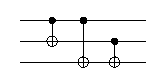
\includegraphics[scale=2]{Figures/circuits/bothEndsSimple}};  
      \node[above left=4.5mm and -7mm of circuit.west, opacity=0.9] {\footnotesize \(A\)};
      \node[left=-7mm of circuit.west, opacity=0.9] {\footnotesize \(B\)};
      \node[below left=4.5mm and -7mm of circuit.west, opacity=0.9] {\footnotesize \(C\)};
      \node[above right=0.8mm and 12.8mm of circuit.west, opacity=0.9] {\footnotesize \(\gamma\)};
      \node[below right=0.8mm and 23.6mm of circuit.west, opacity=0.9] {\footnotesize \(\beta\)};
      \node[below right=0.8mm and 34.4mm of circuit.west, opacity=0.9] {\footnotesize \(\alpha\)};
      \node[right=-3mm of circuit.north west, font=\itshape] (text) {Input:};
    \end{tikzpicture}
  };
  \node[right=3mm of circ] (step1) {
    \begin{tikzpicture}
      \coordinate (O) at (0,0);
      \coordinate (auxA) at (90:9mm);
      \coordinate (auxC) at (330:9mm);
      \coordinate (A) at (90:18mm);
      \coordinate (B) at (210:18mm);
      \coordinate (C) at (330:18mm);
      \coordinate (a) at (270:9mm);
      \coordinate (b) at (30:9mm);
      \coordinate (c) at (150:9mm);
      \draw (auxA) -- (A);
      %\draw (auxA) -- (b);
      \draw (auxA) -- (c);
      %\draw[ultra thick] (auxC) -- (C);
      %\draw[ultra thick] (auxC) -- (b);
      %\draw[ultra thick] (auxC) -- (a);
      %\draw (B) -- (a);
      %\draw[ultra thick] (B) -- (c);
      \node[circle, right=-2.5mm of A, fill=white, inner sep=0pt, minimum size=5mm] {\(A\)};
      %\node[circle, right=-2.5mm of B, fill=white, inner sep=0pt, minimum size=5mm] {\(B\)};
      %\node[circle, right=-2.5mm of C, fill=white, inner sep=0pt, minimum size=5mm] {\(C\)};
      %\node[circle, right=-2.5mm of a, fill=white, inner sep=0pt, minimum size=5mm] {\(\alpha\)};
      %\node[circle, right=-2.5mm of b, fill=white, inner sep=0pt, minimum size=5mm] {\(\beta\)};
      \node[circle, right=-2.5mm of c, fill=white, inner sep=0pt, minimum size=5mm] {\(\gamma\)};
      \node[above left=0mm and 13mm of A, font=\itshape] (text) {1)};
    \end{tikzpicture}
  };
  \node[right=16.5mm of step1] (step2) {
    \begin{tikzpicture}
      \coordinate (O) at (0,0);
      \coordinate (auxA) at (90:9mm);
      \coordinate (auxC) at (330:9mm);
      \coordinate (A) at (90:18mm);
      \coordinate (B) at (210:18mm);
      \coordinate (C) at (330:18mm);
      \coordinate (a) at (270:9mm);
      \coordinate (b) at (30:9mm);
      \coordinate (c) at (150:9mm);
      \draw (auxA) -- (A);
      \draw (auxA) -- (b);
      \draw (auxA) -- (c);
      %\draw[ultra thick] (auxC) -- (C);
      %\draw[ultra thick] (auxC) -- (b);
      %\draw[ultra thick] (auxC) -- (a);
      %\draw (B) -- (a);
      %\draw[ultra thick] (B) -- (c);
      \node[circle, right=-2.5mm of A, fill=white, inner sep=0pt, minimum size=5mm] {\(A\)};
      %\node[circle, right=-2.5mm of B, fill=white, inner sep=0pt, minimum size=5mm] {\(B\)};
      %\node[circle, right=-2.5mm of C, fill=white, inner sep=0pt, minimum size=5mm] {\(C\)};
      %\node[circle, right=-2.5mm of a, fill=white, inner sep=0pt, minimum size=5mm] {\(\alpha\)};
      \node[circle, right=-2.5mm of b, fill=white, inner sep=0pt, minimum size=5mm] {\(\beta\)};
      \node[circle, right=-2.5mm of c, fill=white, inner sep=0pt, minimum size=5mm] {\(\gamma\)};
      \node[above left=0mm and 13mm of A, font=\itshape] (text) {2)};
    \end{tikzpicture}
  };
  \node[below left=5mm and -30mm of circ] (step3) {
    \begin{tikzpicture}
      \coordinate (O) at (0,0);
      \coordinate (auxA) at (90:9mm);
      \coordinate (auxC) at (330:9mm);
      \coordinate (A) at (90:18mm);
      \coordinate (B) at (210:18mm);
      \coordinate (C) at (330:18mm);
      \coordinate (a) at (270:9mm);
      \coordinate (b) at (30:9mm);
      \coordinate (c) at (150:9mm);
      \draw (auxA) -- (A);
      \draw (auxA) -- (b);
      \draw (auxA) -- (c);
      %\draw[ultra thick] (auxC) -- (C);
      %\draw[ultra thick] (auxC) -- (b);
      %\draw[ultra thick] (auxC) -- (a);
      %\draw (B) -- (a);
      \draw[ultra thick] (B) -- (c);
      \node[circle, right=-2.5mm of A, fill=white, inner sep=0pt, minimum size=5mm] {\(A\)};
      \node[circle, right=-2.5mm of B, fill=white, inner sep=0pt, minimum size=5mm] {\(B\)};
      %\node[circle, right=-2.5mm of C, fill=white, inner sep=0pt, minimum size=5mm] {\(C\)};
      %\node[circle, right=-2.5mm of a, fill=white, inner sep=0pt, minimum size=5mm] {\(\alpha\)};
      \node[circle, right=-2.5mm of b, fill=white, inner sep=0pt, minimum size=5mm] {\(\beta\)};
      \node[circle, right=-2.5mm of c, fill=white, inner sep=0pt, minimum size=5mm] {\(\gamma\)};
      \node[above left=0mm and 13mm of A, font=\itshape] (text) {3)};
    \end{tikzpicture}
  };
  \node[right=20mm of step3] (step4) {
    \begin{tikzpicture}
      \coordinate (O) at (0,0);
      \coordinate (auxA) at (90:9mm);
      \coordinate (auxC) at (330:9mm);
      \coordinate (A) at (90:18mm);
      \coordinate (B) at (210:18mm);
      \coordinate (C) at (330:18mm);
      \coordinate (a) at (270:9mm);
      \coordinate (b) at (30:9mm);
      \coordinate (c) at (150:9mm);
      \draw (auxA) -- (A);
      \draw (auxA) -- (b);
      \draw (auxA) -- (c);
      %\draw[ultra thick] (auxC) -- (C);
      %\draw[ultra thick] (auxC) -- (b);
      %\draw[ultra thick] (auxC) -- (a);
      \draw (B) -- (a);
      \draw[ultra thick] (B) -- (c);
      \node[circle, right=-2.5mm of A, fill=white, inner sep=0pt, minimum size=5mm] {\(A\)};
      \node[circle, right=-2.5mm of B, fill=white, inner sep=0pt, minimum size=5mm] {\(B\)};
      %\node[circle, right=-2.5mm of C, fill=white, inner sep=0pt, minimum size=5mm] {\(C\)};
      \node[circle, right=-2.5mm of a, fill=white, inner sep=0pt, minimum size=5mm] {\(\alpha\)};
      \node[circle, right=-2.5mm of b, fill=white, inner sep=0pt, minimum size=5mm] {\(\beta\)};
      \node[circle, right=-2.5mm of c, fill=white, inner sep=0pt, minimum size=5mm] {\(\gamma\)};
      \node[above left=0mm and 13mm of A, font=\itshape] (text) {4)};
    \end{tikzpicture}
  };
  \node[right=20mm of step4] (final) {
    \begin{tikzpicture}
      \coordinate (O) at (0,0);
      \coordinate (auxA) at (90:9mm);
      \coordinate (auxC) at (330:9mm);
      \coordinate (A) at (90:18mm);
      \coordinate (B) at (210:18mm);
      \coordinate (C) at (330:18mm);
      \coordinate (a) at (270:9mm);
      \coordinate (b) at (30:9mm);
      \coordinate (c) at (150:9mm);
      \draw (auxA) -- (A);
      \draw (auxA) -- (b);
      \draw (auxA) -- (c);
      \draw[ultra thick] (auxC) -- (C);
      \draw[ultra thick] (auxC) -- (b);
      \draw[ultra thick] (auxC) -- (a);
      \draw (B) -- (a);
      \draw[ultra thick] (B) -- (c);
      \node[circle, right=-2.5mm of A, fill=white, inner sep=0pt, minimum size=5mm] {\(A\)};
      \node[circle, right=-2.5mm of B, fill=white, inner sep=0pt, minimum size=5mm] {\(B\)};
      \node[circle, right=-2.5mm of C, fill=white, inner sep=0pt, minimum size=5mm] {\(C\)};
      \node[circle, right=-2.5mm of a, fill=white, inner sep=0pt, minimum size=5mm] {\(\alpha\)};
      \node[circle, right=-2.5mm of b, fill=white, inner sep=0pt, minimum size=5mm] {\(\beta\)};
      \node[circle, right=-2.5mm of c, fill=white, inner sep=0pt, minimum size=5mm] {\(\gamma\)};
      \node[above left=0mm and 13mm of A, font=\itshape] (text) {5)};
    \end{tikzpicture}
  };
\end{tikzpicture}
\vspace*{0mm}
\caption{Step by step execution of Algorithm~\ref{code:buildHypBothEnds}.}
\label{fig:BothEndsProcess}
\end{figure}

Algorithm~\ref{code:buildHypBothEnds} builds, for any circuit, a hypergraph that satisfies these requirements. Figure~\ref{fig:BothEndsProcess} shows how the hypergraph from Figure~\ref{fig:BothEndsChallenge}\textit{d)} is built step by step. The three requirements above are satisfied: First, we include all of the control-hyperedges (those from Figure~\ref{fig:BothEndsChallenge}\textit{b)}) and target-hyperedges (those from Figure~\ref{fig:BothEndsChallenge}\textit{c)}). For the second requirement, we give additional structure to the hypergraph, adding vertices that represent CNOT gates. The way a CNOT is implemented will be determined by the block its CNOT-vertex is assigned to. The third requirement is the most subtle one. Intuitively, we satisfy it by imposing that each CNOT-vertex participates in only two hyperedges; one connecting it to its control wire-vertex, the other to its target. A more detailed account of how this third requirement holds is given in the proof of Theorem~\ref{thm:bothEnds}. Corollary~\ref{col:bothEnds} confirms that the optimal partition of our hypergraph determines the most efficient circuit distribution.


\begin{theorem}
 Given any circuit \(\mathcal{C}\), and its hypergraph \(\mathcal{H}\) generated by Algorithm~\ref{code:buildHypBothEnds}, there is a bijection between partitions of \(\mathcal{H}\) with \(\lambda_c\) cuts and distributions of \(\mathcal{C}\) that use \(\lambda_e\) ebits.
 \label{thm:bothEnds}
\end{theorem}
\begin{proof}
We define the same trivial configuration from Theorem~\ref{thm:vanilla}. In the case of the vanilla algorithm (\S\ref{Vanilla}), the CNOT operation itself was always applied in the same QPU as its target, regardless of the CNOT being local or not (see Figure~\ref{fig:nonlocalCNOTs}). Thus, the primitive from Theorem~\ref{thm:vanilla} for reallocating a wire-vertex \(x\) is defined here with the extra constraint that all CNOT-vertices connected by a target-hyperedge to \(x\) must move with it to the same block/QPU \(x\) does. In this way, the primitive has on our new hypergraph representation the exact same meaning it had in the original. 

We need to add another primitive that allows us to move a CNOT-vertex \(x\) independently from its wire-vertices; otherwise not every hypergraph partition would be reachable. Conversely, in order to reach any arbitrary circuit distribution, we need a primitive that changes the QPU where a CNOT gate \(x\) is implemented, which determines the method used to implement the CNOT. This pair of primitives is defined to correspond one-to-one to each other. Let's consider the four distinct cases of how \(x\) may be allocated regarding its two neighbour wire-vertices, which  act as \(x\)'s control \(c_x\) and its target \(t_x\):
\begin{itemize}
  \item \textit{Local}: The three vertices \(x\), \(c_x\) and \(t_x\) are in the same block \(i\). In this case, \(x\)'s allocation causes \textit{no cut} to either its control-hyperedge or its target-hyperedge. The CNOT gate is implemented locally in QPU \(i\), so \textit{no ebit} is required to implement it.

  \item \textit{Remote-control}: Both \(x\) and \(t_x\) are in a block \(i\), while \(c_x\) is in a different block \(j\). In this case, \(x\)'s allocation causes its control-hyperedge to be cut. The cut will be already present if there are other vertices from the hyperedge allocated to \(i\); otherwise \textit{one cut} will be added. On the other hand, an ebit is required to implement CNOT \(x\). If there are other CNOTs in \(i\) controlled by the same \(c_x\) wire -- they are in the same control-hyperedge --, the ebit they require can be used to implement \(x\); otherwise \textit{one ebit} will be added.

  \item \textit{Remote-target}: Both \(x\) and \(c_x\) are in a block \(i\), while \(t_x\) is in a different block \(j\). In this case, \(x\)'s allocation causes its target-hyperedge to be cut. Again, the cut will be already present if there are other vertices from the hyperedge allocated to \(i\); otherwise \textit{one cut} will be added. On the other hand, an ebit is required to implement CNOT \(x\). If there are other CNOTs in \(i\) that target the same \(t_x\) wire -- they are in the same target-hyperedge --, the ebit they require can be used to implement \(x\); otherwise \textit{one ebit} will be added.

  \item \textit{External}: The three vertices are in separated blocks, with \(x\) in some block \(i\). An example of this situation is shown in Figure~\ref{fig:farCNOT}. In this case, \(x\)'s allocation contributes to \textit{two cuts}, one on its control-hyperedge and another on its target-hyperedge. In this case, \textit{two ebits} are required; the one used to access \(c_x\) may be shared with other CNOT gates in \(i\) that have \(c_x\) as control, while the ebit used to access \(t_x\) may be shared with CNOTs in \(i\) that have \(t_x\) as target.
\end{itemize} 

The proof by induction discussed in Theorem~\ref{thm:vanilla} holds here too if we manage to show that any application of the new CNOT-vertex reallocation primitive still preserves \(\lambda_c = \lambda_e\). Changing the allocation of a CNOT-vertex \(x\) may change its situation among the four cases above. As we detailed, in each case \(x\)'s allocation contributes to the same amount of cuts as ebits the CNOT \(x\) requires. Hence, changing the allocation of \(x\) always preserves \(\lambda_c = \lambda_e\).

\end{proof}

\begin{figure}[h]
\hspace*{-8mm}
\begin{tikzpicture}
  \node (circ) {
    \begin{tikzpicture}
      \node[inner sep=0pt] (circuit) {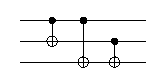
\includegraphics[scale=2]{Figures/circuits/bothEndsSimple}};  
      \node[above left=4.5mm and -7mm of circuit.west, opacity=0.9] {\footnotesize \(A\)};
      \node[left=-7mm of circuit.west, opacity=0.9] {\footnotesize \(B\)};
      \node[below left=4.5mm and -7mm of circuit.west, opacity=0.9] {\footnotesize \(C\)};
      \node[above right=0.8mm and 12.8mm of circuit.west, opacity=0.9] {\footnotesize \(\gamma\)};
      \node[below right=0.8mm and 23.6mm of circuit.west, opacity=0.9] {\footnotesize \(\beta\)};
      \node[below right=0.8mm and 34.4mm of circuit.west, opacity=0.9] {\footnotesize \(\alpha\)};
      \node[right=-3mm of circuit.north west, font=\itshape] (text) {a)};
    \end{tikzpicture}
  };
  \node[below right=-40mm and 20mm of circ] (hypergraph) {
    \begin{tikzpicture}
      \coordinate (O) at (0,0);
      \coordinate (auxA) at (90:9mm);
      \coordinate (auxC) at (330:9mm);
      \coordinate (A) at (90:18mm);
      \coordinate (B) at (210:18mm);
      \coordinate (C) at (330:18mm);
      \coordinate (a) at (270:9mm);
      \coordinate (b) at (30:9mm);
      \coordinate (c) at (150:9mm);
      \draw (auxA) -- (A);
      \draw (auxA) -- (b);
      \draw (auxA) -- (c);
      \draw[ultra thick] (auxC) -- (C);
      \draw[ultra thick] (auxC) -- (b);
      \draw[ultra thick] (auxC) -- (a);
      \draw (B) -- (a);
      \draw[ultra thick] (B) -- (c);
      \node[circle, right=-2.5mm of A, fill=white, inner sep=0pt, minimum size=5mm] {\(A\)};
      \node[circle, right=-2.5mm of B, fill=white, inner sep=0pt, minimum size=5mm] {\(B\)};
      \node[circle, right=-2.5mm of C, fill=white, inner sep=0pt, minimum size=5mm] {\(C\)};
      \node[circle, right=-2.5mm of a, fill=white, inner sep=0pt, minimum size=5mm] {\(\alpha\)};
      \node[circle, right=-2.5mm of b, fill=white, inner sep=0pt, minimum size=5mm] {\(\beta\)};
      \node[circle, right=-2.5mm of c, fill=white, inner sep=0pt, minimum size=5mm] {\(\gamma\)};
      \coordinate (joinPoint) at (30:15.5mm);
      \coordinate (leftPoint) at (300:16mm);
      \pic (cut) {cut=leftPoint/joinPoint};
      \coordinate (leftPoint2) at (120:16mm);
      \pic (cut2) {cut=leftPoint2/joinPoint};
      \coordinate (extraPoint) at (30:23.5mm);
      \pic (cut3) {cut=extraPoint/joinPoint};
      \node[above left=0mm and 13mm of A, font=\itshape] (text) {b)};
    \end{tikzpicture}
  };
  \node[below right=5mm and -70mm of circ] (distributed) {
    \begin{tikzpicture}
      \node[inner sep=0pt] (circuit) {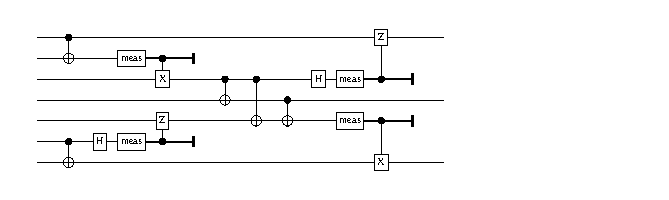
\includegraphics[scale=2]{Figures/circuits/farCNOTDistrib}};  
      \pic (e1) {ebit=e1/12.7mm/13mm};
      \pic (e2) {ebit=e2/33.84mm/13mm};
      \node[above left=18.58mm and -7mm of circuit.west, opacity=0.9] {\footnotesize \(A\)};
      \node[left=-7mm of circuit.west, opacity=0.9] {\footnotesize \(B\)};
      \node[below left=18.58mm and -7mm of circuit.west, opacity=0.9] {\footnotesize \(C\)};
      \node[above right=0.8mm and 65.8mm of circuit.west, opacity=0.9] {\footnotesize \(\gamma\)};
      \node[below right=0.8mm and 76.6mm of circuit.west, opacity=0.9] {\footnotesize \(\beta\)};
      \node[below right=0.8mm and 87.4mm of circuit.west, opacity=0.9] {\footnotesize \(\alpha\)};
      \coordinate[above left=10.5mm and -5mm of circuit.west] (leftPoint1);
      \coordinate[right=142mm of leftPoint1] (rightPoint1);
      \pic (cut1) {cut=leftPoint1/rightPoint1};
      \coordinate[below left=10.5mm and -5mm of circuit.west] (leftPoint2);
      \coordinate[right=142mm of leftPoint2] (rightPoint2);
      \pic (cut2) {cut=leftPoint2/rightPoint2};
      \node[right=-3mm of circuit.north west, font=\itshape] (text) {c)};
    \end{tikzpicture}
  };
\end{tikzpicture}
\caption{Distribution of circuit \textit{a)} when each wire is in a different QPU. Gate \(\beta\) is implemented as an `external' CNOT, i.e.\ both its control and target are in a remote QPU.}
\label{fig:farCNOT}
\end{figure}

The procedure for distributing the circuit following a given hypergraph partition is very similar to that in the vanilla version of the algorithm, now taking into account the new primitive defined in Theorem~\ref{thm:bothEnds}. The time complexity of the procedure still is \(O(n\cdot m)\), where \(n\) is the total number of vertices and \(m\) is the number of hyperedges. Also, notice that the cat-entangler and the cat-disentangler are slightly different whether the CNOTs are implemented through remote-control or remote-target (see Figure~\ref{fig:farCNOT}).

\begin{corollary}
The best distribution of a circuit can be efficiently derived from an optimal partition of the hypergraph built by Algorithm~\ref{code:buildHypBothEnds}.
\label{col:bothEnds}
\end{corollary}
\begin{proof}
Follows directly from Theorem~\ref{thm:bothEnds}, by the same argument given for Corollary~\ref{col:vanilla}. 

\end{proof}

\begin{corollary}
The distributed circuit we obtain using the vanilla algorithm (from \S\ref{Vanilla}) is the same as the one obtained if we restrict the approach in this subsection so either:
\begin{enumerate}
  \renewcommand{\theenumi}{\alph{enumi})}
  \item No CNOT is implemented using the remote-target method.
  \item Our hypergraph partitioner never cuts target-hyperedges.
  \item The CNOT operation is always executed in the CNOT's target QPU.
\end{enumerate}
All of these restrictions are equivalent.
\end{corollary}
\begin{proof}
Follows directly from the proof of Theorem~\ref{thm:bothEnds}.

\end{proof}

The hypergraph built by Algorithm~\ref{code:buildHypBothEnds} has one caveat: When discussing load-balancing in \S\ref{EfficientDistrib}, we explained that we were interested in allocating a uniform number of wires to each QPU. Previously, the hypergraph partitioner took care of this, as it tried to assign a uniform number of vertices to each block. But now, the hypergraph partitioner has no way of distinguishing between `wire' vertices and `CNOT' vertices, the latter being an artificial gadget that should not count towards load-balancing. The solution is simple, instead of the standard hypergraph partition problem, we apply a version of it where vertices can have a weight assigned (see Appendix~\ref{chap:HypPart}). Then, each wire-vertex is given weight \(1\), and each CNOT-vertex is given weight \(0\), effectively ignoring them for the load-balancing aspect.

\begin{remark} 
Enabling \texttt{EitherRemote} will never increase the ebit count required to implement a partition.

\normalfont
This extension simply changes how each non-local CNOT is implemented, while the number of non-local CNOTs remains the same. On the worst case, these non-local CNOTs could be implemented in the exact same way as they were before, so the ebit count would remain the same.

\label{thm:BothEndsImprove}
\end{remark}

The case illustrated in Figure~\ref{fig:farCNOT} can be seen intuitively as passing a message through a middle-man. Sometimes, using communication through an already available middle-man is better than putting up a full blown connection just for a single message. The hypergraph partitioner acting on the hypergraph built by Algorithm~\ref{code:buildHypBothEnds} will automatically use this strategy whenever it reduces the number of ebits required. However, some criticism is relevant here: if we put no constraint on the exploitation of `middle-men' QPUs, it may happen that communication across many of the QPUs all use the same middle-man QPU to deliver their messages, potentially creating a bottle neck. We see two solutions:

%Notice, however, that this trick only allows to implement a single CNOT with both target and control wires in some particular QPUs. When the CNOT shares one of its wires with multiple CNOTs, it will often be best to use the remote-control or remote-target method to implement all of them together. This trick will be useful whenever there are stray CNOT gates that can not be efficiently grouped with other CNOTs.

\begin{enumerate}
\item Specialise the hardware to be efficiently managed as a centralised communication network, where the middle-man QPU has a similar role to a classical server. The server should be capable of managing a large number of ebits fast and reliably. This is the natural option if the algorithms we wish to run have an intrinsically centralised behaviour -- for instance, if all the gates are controlled by the same wire.

\item In case we wish to have a decentralised network, we will need to find a way to ensure the hypergraph partition we get has some kind of load-balancing of the usage of ebits. Fortunately, there is a simple way to do this: instead of giving CNOT vertices weight \(0\) as we previously discussed, we may give them some weight \(\mu > 0\) that indicates how relevant communication load-balancing is in comparison to the load-balancing of wire allocation across QPUs. Alternatively, we could use a custom version of the hypergraph partitioning problem where we provide three parameters instead of two, \((k,\varepsilon,\eta)\), where now \(\varepsilon\) acts only as the tolerance for imbalance of wire-vertices, while \(\eta\) is a separate tolerance for imbalance of CNOT-vertices, both tolerances being enforced at any partition.
\end{enumerate}

The best choice between either of the above options, and the selection of a suitable value for \(\mu\) or \(\eta\), will be dependent on the algorithms we intend to run. However, users may not know beforehand which configuration is best for their algorithms. This problem also exists in classical computer science, as the effectiveness of many compiler optimisations depend on the choice of the parameter configuration. In those cases, compiler writers tend to follow one of two solutions: One option is to include a decision algorithm in the compiler's code, that looks at particular characteristics of the input and chooses a suitable parameter configuration for its compilation. Another option is to provide a default configuration that does a reasonable job in most cases, and leave the task of fine-tuning to the user, who should compile the program multiple times with different configurations until the best one is found. Making a decision on which approach to use requires a thorough study of the effects of each parameter on a diverse benchmark. We include this study in our list of suggestions for further work (see \S\ref{FurtherWork}).

%Across the figures of this subsection we have drawn differently hyperedges that group CNOTs with remote-control or remote-target. However, it should be noticed that the hypergraph partitioner does not use this information at any point. This distinction is made for explanation purposes, and it is only relevant when building the distributed version of the circuit. 

As a wrap up for this section, Figure~\ref{fig:modes} shows the same circuit being distributed in four different ways: with or without \texttt{SlideCNOTs} and with or without \texttt{EitherRemote}. This provides a simple example where both extensions are shown to reduce the number of ebits required to distribute a circuit.

\begin{figure}
\centering
\begin{tikzpicture}
  \node (input) {
    \begin{tikzpicture}
      \node[inner sep=0pt] (circuit) {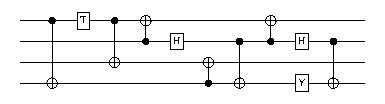
\includegraphics[scale=2]{Figures/circuits/interesting}};  
      \node[above left=8mm and -7mm of circuit.west, opacity=0.9] {\footnotesize \(A\)};
      \node[above left=1mm and -7mm of circuit.west, opacity=0.9] {\footnotesize \(B\)};
      \node[below left=1mm and -7mm of circuit.west, opacity=0.9] {\footnotesize \(C\)};
      \node[below left=8mm and -7mm of circuit.west, opacity=0.9] {\footnotesize \(D\)};
      \node[below right=4.3mm and 12.8mm of circuit.west, opacity=0.9] {\footnotesize \(\alpha\)};
      \node[right=0.8mm and 34.4mm of circuit.west, opacity=0.9] {\footnotesize \(\beta\)};
      \node[above right=4.3mm and 44.7mm of circuit.west, opacity=0.9] {\footnotesize \(\gamma\)};
      \node[below right=4.3mm and 65.8mm of circuit.west, opacity=0.9] {\footnotesize \(\delta\)};
      \node[below right=4.3mm and 76.4mm of circuit.west, opacity=0.9] {\footnotesize \(\eta\)};
      \node[above right=4.3mm and 87.0mm of circuit.west, opacity=0.9] {\footnotesize \(\theta\)};
      \node[below right=4.3mm and 108.4mm of circuit.west, opacity=0.9] {\footnotesize \(\mu\)};
      \node[right=-3mm of circuit.north west, font=\itshape] (text) {Input:};
    \end{tikzpicture}
  };
  \node[below=5mm of input] (pulled) {
    \begin{tikzpicture}
      \node[inner sep=0pt] (circuit) {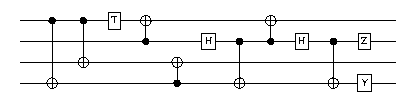
\includegraphics[scale=2]{Figures/circuits/interestingPulled}};  
      \node[above left=8mm and -7mm of circuit.west, opacity=0.9] {\footnotesize \(A\)};
      \node[above left=1mm and -7mm of circuit.west, opacity=0.9] {\footnotesize \(B\)};
      \node[below left=1mm and -7mm of circuit.west, opacity=0.9] {\footnotesize \(C\)};
      \node[below left=8mm and -7mm of circuit.west, opacity=0.9] {\footnotesize \(D\)};
      \node[below right=4.3mm and 12.8mm of circuit.west, opacity=0.9] {\footnotesize \(\alpha\)};
      \node[right=0.8mm and 24.2mm of circuit.west, opacity=0.9] {\footnotesize \(\beta\)};
      \node[above right=4.3mm and 44.7mm of circuit.west, opacity=0.9] {\footnotesize \(\gamma\)};
      \node[below right=4.3mm and 56.1mm of circuit.west, opacity=0.9] {\footnotesize \(\delta\)};
      \node[below right=4.3mm and 76.4mm of circuit.west, opacity=0.9] {\footnotesize \(\eta\)};
      \node[above right=4.3mm and 87.0mm of circuit.west, opacity=0.9] {\footnotesize \(\theta\)};
      \node[below right=4.3mm and 108.4mm of circuit.west, opacity=0.9] {\footnotesize \(\mu\)};
      \node[right=-3mm of circuit.north west, font=\itshape] (text) {After preprocessing (extension from \S\ref{pullCNOTs}):};
    \end{tikzpicture}
  };
  \node[below left=5mm and -60mm of pulled] (FF) {
    \begin{tikzpicture}
      \coordinate (A) at (135:22mm);
      \coordinate (B) at (45:22mm);
      \coordinate (C) at (225:22mm);
      \coordinate (D) at (315:22mm);
      \coordinate[below left=12mm and 12mm of B] (auxB);
      \draw (C) -- (A);
      \draw (A) edge[out=290,in=160] (D);
      \draw (B) -- (auxB);
      \draw (A) -- (auxB);
      \draw (D) -- (auxB);
      \draw (A) -- (B);
      \draw (D) -- (B);
      \draw (C) -- (D);
      \node[circle, right=-2.5mm of A, fill=white, inner sep=0pt, minimum size=5mm] {\(A\)};
      \node[circle, right=-2.5mm of B, fill=white, inner sep=0pt, minimum size=5mm] {\(B\)};
      \node[circle, right=-2.5mm of C, fill=white, inner sep=0pt, minimum size=5mm] {\(C\)};
      \node[circle, right=-2.5mm of D, fill=white, inner sep=0pt, minimum size=5mm] {\(D\)};
      \coordinate[below left=20mm and 4mm of A] (p0);
      \coordinate[below right=20mm and 4mm of B] (p1);
      \pic (cut) {cut=p0/p1};
      \node[above left=0mm and 8mm of A, font=\itshape] (text) {a)};
    \end{tikzpicture}
  };
  \node[right=15mm of FF] (FT) {
    \begin{tikzpicture}
      \coordinate (A) at (135:22mm);
      \coordinate (B) at (45:22mm);
      \coordinate (C) at (225:22mm);
      \coordinate (D) at (315:22mm);
      \coordinate (a) at (270:7mm);
      \coordinate (b) at (180:18mm);
      \coordinate (c) at (90:18mm);
      \coordinate (d) at (270:18mm);
      \coordinate (e) at (30:7mm);
      \coordinate (t) at (150:7mm);
      \coordinate (m) at (0:18mm);
      \coordinate[above left=5mm and 1mm of t] (auxAt);
      \coordinate[above right=7mm and 1mm of e] (auxB);
      \coordinate[above right=5mm and 5mm of C] (auxC);
      \draw (A) edge[out=290,in=145] (a);
      \draw (b) -- (A);
      \draw[ultra thick] (A) -- (auxAt);
      \draw[ultra thick] (t) -- (auxAt);
      \draw[ultra thick] (c) -- (auxAt);
      \draw (B) -- (auxB);
      \draw (t) -- (auxB);
      \draw (e) -- (auxB);
      \draw[ultra thick] (C) -- (auxC);
      \draw[ultra thick] (b) -- (auxC);
      \draw[ultra thick] (d) -- (auxC);
      \draw[ultra thick] (D) -- (e);
      \draw[ultra thick] (m) -- (D);
      \draw (c) -- (B);
      \draw (m) -- (B);
      \draw[ultra thick] (a) -- (D);
      \draw (d) -- (D);
      \node[circle, right=-2.5mm of A, fill=white, inner sep=0pt, minimum size=5mm] {\(A\)};
      \node[circle, right=-2.5mm of B, fill=white, inner sep=0pt, minimum size=5mm] {\(B\)};
      \node[circle, right=-2.5mm of C, fill=white, inner sep=0pt, minimum size=5mm] {\(C\)};
      \node[circle, right=-2.5mm of D, fill=white, inner sep=0pt, minimum size=5mm] {\(D\)};
      \node[circle, right=-2.5mm of a, fill=white, inner sep=0pt, minimum size=5mm] {\(\alpha\)};
      \node[circle, right=-2.5mm of b, fill=white, inner sep=0pt, minimum size=5mm] {\(\beta\)};
      \node[circle, right=-2.5mm of c, fill=white, inner sep=0pt, minimum size=5mm] {\(\gamma\)};
      \node[circle, right=-2.5mm of d, fill=white, inner sep=0pt, minimum size=5mm] {\(\delta\)};
      \node[circle, right=-2.5mm of e, fill=white, inner sep=0pt, minimum size=5mm] {\(\eta\)};
      \node[circle, right=-2.5mm of t, fill=white, inner sep=0pt, minimum size=5mm] {\(\theta\)};
      \node[circle, right=-2.5mm of m, fill=white, inner sep=0pt, minimum size=5mm] {\(\mu\)};
      \coordinate[above right=4mm and 6.5mm of A] (p0);
      \coordinate[below right=4mm and 6.5mm of C] (p1);
      \pic (cut) {cut=p0/p1};
      %\draw[dash pattern={on 7pt off 2pt on 1pt off 2pt}, line width=1pt, opacity=0.65] (p1) edge[out=0,in=150,looseness=0.7] (p2);
      \node[above left=0mm and 8mm of A, font=\itshape] (text) {b)};
    \end{tikzpicture}
  };
  \node[below=5mm of FF] (TF) {
    \begin{tikzpicture}
      \coordinate (A) at (135:22mm);
      \coordinate (B) at (45:22mm);
      \coordinate (C) at (225:22mm);
      \coordinate (D) at (315:22mm);
      \coordinate[above right=10mm and 10mm of C] (auxAc);
      \coordinate[below left=10mm and 10mm of B] (auxB);
      \draw (A) -- (auxAc);
      \draw (D) -- (auxAc);
      \draw (C) -- (auxAc);
      \draw (B) -- (auxB);
      \draw (A) -- (auxB);
      \draw (D) -- (auxB);
      \draw (A) -- (B);
      \draw (D) -- (B);
      \draw (C) -- (D);
      \node[circle, right=-2.5mm of A, fill=white, inner sep=0pt, minimum size=5mm] {\(A\)};
      \node[circle, right=-2.5mm of B, fill=white, inner sep=0pt, minimum size=5mm] {\(B\)};
      \node[circle, right=-2.5mm of C, fill=white, inner sep=0pt, minimum size=5mm] {\(C\)};
      \node[circle, right=-2.5mm of D, fill=white, inner sep=0pt, minimum size=5mm] {\(D\)};
      \coordinate[below left=10mm and 4mm of A] (p0);
      \coordinate[above right=10mm and 4mm of D] (p1);
      \pic (cut) {cut=p0/p1};
      \node[above left=0mm and 8mm of A, font=\itshape] (text) {c)};
    \end{tikzpicture}
  };
  \node[right=15mm of TF] (TT) {
    \begin{tikzpicture}
      \coordinate (A) at (135:22mm);
      \coordinate (B) at (45:22mm);
      \coordinate (C) at (225:22mm);
      \coordinate (D) at (315:22mm);
      \coordinate (a) at (270:7mm);
      \coordinate (b) at (180:18mm);
      \coordinate (c) at (90:18mm);
      \coordinate (d) at (270:18mm);
      \coordinate (e) at (30:7mm);
      \coordinate (t) at (150:7mm);
      \coordinate (m) at (0:18mm);
      \coordinate[below right=2mm and 9mm of b] (auxAc);
      \coordinate[above left=5mm and 1mm of t] (auxAt);
      \coordinate[above right=7mm and 1mm of e] (auxB);
      \coordinate[above right=5mm and 5mm of C] (auxC);
      \coordinate[below left=5mm and 5mm of m] (auxD);
      \draw (A) -- (auxAc);
      \draw (a) -- (auxAc);
      \draw (b) -- (auxAc);
      \draw[ultra thick] (A) -- (auxAt);
      \draw[ultra thick] (t) -- (auxAt);
      \draw[ultra thick] (c) -- (auxAt);
      \draw (B) -- (auxB);
      \draw (t) -- (auxB);
      \draw (e) -- (auxB);
      \draw[ultra thick] (C) -- (auxC);
      \draw[ultra thick] (b) -- (auxC);
      \draw[ultra thick] (d) -- (auxC);
      \draw[ultra thick] (D) -- (auxD);
      \draw[ultra thick] (e) -- (auxD);
      \draw[ultra thick] (m) -- (auxD);
      \draw (c) -- (B);
      \draw (m) -- (B);
      \draw[ultra thick] (a) -- (D);
      \draw (d) -- (D);
      \node[circle, right=-2.5mm of A, fill=white, inner sep=0pt, minimum size=5mm] {\(A\)};
      \node[circle, right=-2.5mm of B, fill=white, inner sep=0pt, minimum size=5mm] {\(B\)};
      \node[circle, right=-2.5mm of C, fill=white, inner sep=0pt, minimum size=5mm] {\(C\)};
      \node[circle, right=-2.5mm of D, fill=white, inner sep=0pt, minimum size=5mm] {\(D\)};
      \node[circle, right=-2.5mm of a, fill=white, inner sep=0pt, minimum size=5mm] {\(\alpha\)};
      \node[circle, right=-2.5mm of b, fill=white, inner sep=0pt, minimum size=5mm] {\(\beta\)};
      \node[circle, right=-2.5mm of c, fill=white, inner sep=0pt, minimum size=5mm] {\(\gamma\)};
      \node[circle, right=-2.5mm of d, fill=white, inner sep=0pt, minimum size=5mm] {\(\delta\)};
      \node[circle, right=-2.5mm of e, fill=white, inner sep=0pt, minimum size=5mm] {\(\eta\)};
      \node[circle, right=-2.5mm of t, fill=white, inner sep=0pt, minimum size=5mm] {\(\theta\)};
      \node[circle, right=-2.5mm of m, fill=white, inner sep=0pt, minimum size=5mm] {\(\mu\)};
      \coordinate[above=7mm of b] (p1);
      \coordinate[below=4mm of t] (p2);
      \coordinate[below=7mm of m] (p3);
      \coordinate[left=4mm of p1] (p0);
      \coordinate[right=4mm of p3] (p4);
      \draw[dash pattern={on 7pt off 2pt on 1pt off 2pt}, line width=1pt, opacity=0.65] (p0) -- (p1);
      \draw[dash pattern={on 7pt off 2pt on 1pt off 2pt}, line width=1pt, opacity=0.65] (p1) edge[out=0,in=150,looseness=0.7] (p2);
      \draw[dash pattern={on 7pt off 2pt on 1pt off 2pt}, line width=1pt, opacity=0.65] (p2) edge[out=330,in=180,looseness=0.7] (p3);
      \draw[dash pattern={on 7pt off 2pt on 1pt off 2pt}, line width=1pt, opacity=0.65] (p3) -- (p4);
      \node[above left=0mm and 8mm of A, font=\itshape] (text) {d)};
    \end{tikzpicture}
  };
\end{tikzpicture}
\vspace*{2mm}
\caption{Different hypergraphs representing the input circuit. \textit{a)} corresponds to no extensions active. \textit{c)} and \textit{d)} use the extension from \S\ref{pullCNOTs}. \textit{b)} and \textit{d)} use the extension from \S\ref{BothEnds}. For each hypergraph, the optimal \(k=2\) partition is shown. The number of ebits required in each case is: \textit{a)} \(4\), \textit{b)} \(3\), \textit{c)} \(3\), \textit{d)} \(2\).}
\label{fig:modes}
\end{figure}

\section{Interchanging CNOT gates}
\label{Interchange}

In this section we discuss a potential improvement to our algorithm. We focus on explaining the challenges it implies, and we outline an approach to tackle them. Overall, this section should be understood as a draft idea for future work. 

When applied to disjoint sets of wires, CNOT gates commute trivially. If one of the wires is in common, and it has the same role for both CNOTs (control or target), we can implement both gates using a single ebit. If both wires are in common and have the same role, the CNOTs cancel each other. But what happens if two CNOTs act on the same wire with different roles? In that case, we can still interchange the gates as in Figure~\ref{fig:interchangeRule}, but this creates an additional CNOT.

\begin{figure}
\centering
\begin{tikzpicture}
  \node {
    \begin{tikzpicture}
      \node[inner sep=0pt] (circuit) at (0,0) {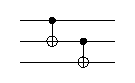
\includegraphics[scale=2]{Figures/circuits/interchangeCNOTs1}};
      \node[right=0mm of circuit.north west, font=\itshape] (text) {a)};
    \end{tikzpicture}
    \hspace{8mm}
    \begin{tikzpicture}
      \node[inner sep=0pt] (circuit) at (0,0) {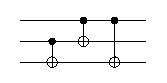
\includegraphics[scale=2]{Figures/circuits/interchangeCNOTs2}};
      \node[right=0mm of circuit.north west, font=\itshape] (text) {b)};
    \end{tikzpicture}
  };
\end{tikzpicture}
\caption{Equivalent circuits with the two gates in \textit{a)} being interchanged in \textit{b)}. A byproduct CNOT gate is created in the process.}
\label{fig:interchangeRule}
\end{figure}

\begin{figure}[h]
\centering
\begin{tikzpicture}
  \node (circ) {
    \begin{tikzpicture}
      \node[inner sep=0pt] (circuit) {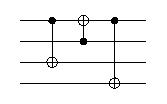
\includegraphics[scale=2, trim={2.5mm 0 2.5mm 0}, clip]{Figures/circuits/interchangeChallenge1}};  
      \node[left=-7mm of circuit.west, rectangle,fill=white,minimum height=22mm, minimum width=8mm] {};
      \node[right=-7mm of circuit.east, rectangle,fill=white,minimum height=22mm, minimum width=8mm] {};
      \node[above left=8mm and -7mm of circuit.west, opacity=0.9] {\footnotesize \(A\)};
      \node[above left=1mm and -7mm of circuit.west, opacity=0.9] {\footnotesize \(B\)};
      \node[below left=1mm and -7mm of circuit.west, opacity=0.9] {\footnotesize \(C\)};
      \node[below left=8mm and -7mm of circuit.west, opacity=0.9] {\footnotesize \(D\)};
      \coordinate[above left=7.2mm and -6mm of circuit.west] (leftPoint);
      \coordinate[above right=7.2mm and -6mm of circuit.east] (rightPoint);
      \pic (cut) {cut=leftPoint/rightPoint};
      \node[right=-3mm of circuit.north west, font=\itshape] (text) {a)};
    \end{tikzpicture}
  };
  \node[below=5mm of circ] (interchanged) {
    \begin{tikzpicture}
      \node[inner sep=0pt] (circuit) {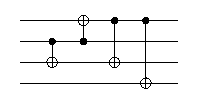
\includegraphics[scale=2, trim={2.5mm 0 2.5mm 0}, clip]{Figures/circuits/interchangeChallenge2}};  
      \node[left=-7mm of circuit.west, rectangle,fill=white,minimum height=22mm, minimum width=8mm] {};
      \node[right=-7mm of circuit.east, rectangle,fill=white,minimum height=22mm, minimum width=8mm] {};
      \node[right=-3mm of circuit.north west, font=\itshape] (text) {c)};
      \node[above left=8mm and -7mm of circuit.west, opacity=0.9] {\footnotesize \(A\)};
      \node[above left=1mm and -7mm of circuit.west, opacity=0.9] {\footnotesize \(B\)};
      \node[below left=1mm and -7mm of circuit.west, opacity=0.9] {\footnotesize \(C\)};
      \node[below left=8mm and -7mm of circuit.west, opacity=0.9] {\footnotesize \(D\)};
      \coordinate[above left=7.2mm and -6mm of circuit.west] (leftPoint);
      \coordinate[above right=7.2mm and -6mm of circuit.east] (rightPoint);
      \pic (cut) {cut=leftPoint/rightPoint};
      \node[right=-3mm of circuit.north west, font=\itshape] (text) {c)};
    \end{tikzpicture}
  };
  \node[above right=-38mm and 15mm of circ] (hypergraph) {
    \begin{tikzpicture}
      \coordinate (B) at (45:15mm);
      \coordinate (A) at (135:15mm);
      \coordinate (C) at (225:15mm);
      \coordinate (D) at (0,0);
      \draw (A) -- (C);
      \draw (A) -- (B);
      \draw (A) -- (D);
      \node[circle, right=-2.5mm of A, fill=white, inner sep=0pt, minimum size=5mm] {\(A\)};
      \node[circle, right=-2.5mm of B, fill=white, inner sep=0pt, minimum size=5mm] {\(B\)};
      \node[circle, right=-2.5mm of C, fill=white, inner sep=0pt, minimum size=5mm] {\(C\)};
      \node[circle, right=-2.5mm of D, fill=white, inner sep=0pt, minimum size=5mm] {\(D\)};
      \coordinate (leftPoint) at (195:15mm);
      \coordinate (rightPoint) at (75:15mm);
      \pic (cut) {cut=leftPoint/rightPoint};
      \node[above left=5mm and 9mm of A, font=\itshape] (text) {b)};
    \end{tikzpicture}
  };
  \node[below=8.5mm of hypergraph] (hypergraph2) {
    \begin{tikzpicture}
      \coordinate (B) at (45:15mm);
      \coordinate (A) at (135:15mm);
      \coordinate (C) at (225:15mm);
      \coordinate (D) at (0,0);
      \coordinate (aux) at (180:6.5mm);
      \draw (A) -- (B);
      \draw (B) to [bend left] (C);
      \draw (aux) -- (A);
      \draw (aux) -- (C);
      \draw (aux) -- (D);
      \node[circle, right=-2.5mm of A, fill=white, inner sep=0pt, minimum size=5mm] {\(A\)};
      \node[circle, right=-2.5mm of B, fill=white, inner sep=0pt, minimum size=5mm] {\(B\)};
      \node[circle, right=-2.5mm of C, fill=white, inner sep=0pt, minimum size=5mm] {\(C\)};
      \node[circle, right=-2.5mm of D, fill=white, inner sep=0pt, minimum size=5mm] {\(D\)};
      \coordinate (leftPoint) at (195:15mm);
      \coordinate (rightPoint) at (75:15mm);
      \pic (cut) {cut=leftPoint/rightPoint};
      \node[above left=5mm and 9mm of A, font=\itshape] (text) {d)};
    \end{tikzpicture}
  };
\end{tikzpicture}
\vspace*{5mm}
\caption{Example of a circuit \textit{a)} where interchanging the first two gates saves an ebit for the proposed partition. The byproduct gate in circuit \textit{c)} will be implemented locally, so its addition has no impact. Two of the CNOTs in \textit{c)} can be implemented using a single ebit. Hypergraph \textit{b)} corresponds to the circuit \textit{a)}. Hypergraph \textit{d)} corresponds to \textit{c)}, and it has one less cut.}
\label{fig:interchangeChallenge}
\end{figure}

It may seem like pre-processing the circuit so it has the minimum possible number of CNOT gates would always be the best option for partitioning. However, this is not always true, as shown in Figure~\ref{fig:interchangeChallenge}. In some cases interchanging CNOTs may unlock a more efficient distribution of the circuit. To account for this, the effect of CNOT interchange should also be encoded in our hypergraph representation. However, encoding that information in a hypergraph is not natural, due to the following reasons:

\begin{itemize}
  \item \textit{The way CNOT gates are ordered in the circuit is important}: This is something we omit in the hypergraphs built by Algorithms~\ref{code:buildHypVanilla} and~\ref{code:buildHypBothEnds}: looking at the final hypergraph in Figure~\ref{fig:BothEndsProcess}, we can not tell whether \(\alpha\) goes before or after \(\beta\). This information is key when interchanging, as it will determine which are the new neighbours of the interchanged CNOTs. A possible approach would be to impose that every hyperedge is an ordered list of vertices\footnote{For instance, the first vertex corresponding to a wire and the rest, corresponding to the different CNOT gates, ordered as in the circuit.}. However, the standard hypergraph partitioning problem does not take into account such ordering. We would need to define a custom hypergraph partitioning problem in order to manage this new aspect.

  \item \textit{Interchanging CNOT gates adds new CNOTs}: The CNOT interchange problem is substantially different from the one we discussed and solved in \S\ref{BothEnds}. The essence of our solution was to represent all of the potential choices in a single hypergraph. However, if were to interchange a pair of CNOTs, new choices would become available: Is it worth to interchange the CNOTs again with their new neighbours? Should the byproduct CNOT be itself interchanged further? Although the number of options to take into account is finite, it increases considerably fast. Furthermore, each choice would not be independent from the rest -- as some interchanges are only available if others have been done before -- so the structure of the hypergraph would likely be quite complex in order to accommodate this information.
\end{itemize}

Instead of encoding this choice within the hypergraph partioning problem, we may abandon the idea of guaranteeing the optimal solution, and approach this problem through pre-processing and post-processing. We suggest that a reasonable approach in that case would be to:
\begin{enumerate} 
\item Apply a pre-processing phase that finds an equivalent circuit whose hypergraph has the minimum possible number of hyperedges. 
\item Apply the procedure described in the previous section, which decides how to partition the circuit. 
\item Apply a post-processing phase that exhaustively explores each possible interchange of CNOTs. Those that reduce the number of ebits required to implement the partition are used.
\end{enumerate}

\textbf{TODO}: Is this a greedy algorithm? (most probably, a greedy algorithm won't be optimal... maybe dynamic programming?) If I have time I should I give more details on the strategy? Maybe implement it.
